\documentclass[a4paper,11pt]{report}

\usepackage{fancyhdr}
\usepackage{graphicx}
\usepackage[top=2.5cm, bottom=2.5cm, left=3.0cm, right=2.5cm]{geometry}
\usepackage{setspace}
\usepackage[linktoc=page]{hyperref}
\usepackage{sectsty}
\chapterfont{\centering}
\usepackage{makeidx}
\usepackage{url}
\usepackage[square,sort,comma,numbers,compress]{natbib}
\usepackage{framed}
\usepackage{longtable}
\usepackage{amsfonts}
\usepackage{amsmath}
\usepackage{booktabs} % For better looking tables
\usepackage{array}
\usepackage{tabularx}
\usepackage{makecell}
% \usepackage[noend,ruled,noline,linesnumbered,algochapter]{algorithm2e} % Uncomment after: sudo apt-get install texlive-science
\usepackage{times}
% \usepackage{indentfirst} — replaced with block paragraph style below
\usepackage{caption}
\usepackage{subcaption}
\usepackage{listings}
\usepackage[table]{xcolor}
\definecolor{ganttgray}{RGB}{160,160,160}
\usepackage{multirow}
\usepackage{tikz}
\usetikzlibrary{shapes.geometric, arrows.meta, positioning, fit, calc}
\usepackage{pgfplots}
\pgfplotsset{compat=1.18}
\usepgfplotslibrary{colorbrewer}

% Header space — fancyhdr requires headheight >= actual header content height
\setlength{\headheight}{14pt}
\setlength{\headsep}{0.6cm}

\begin{document}

% Block paragraph style: no first-line indent, small vertical gap between paragraphs
\setlength{\parindent}{0em}
\setlength{\parskip}{5pt}
% 1.5 line spacing throughout
\setstretch{1.5}

% Fancy header and footer settings
\pagestyle{fancy}
\fancypagestyle{plain}{%
    \fancyhf{} % clear all header and footer fields
    \renewcommand{\headrulewidth}{0pt}
    \fancyfoot[L]{\textit{\textcopyright Daffodil International University}}
    \fancyfoot[R]{\thepage}
}

\fancyhf{} % clear all header and footer fields
\renewcommand{\headrulewidth}{0pt}
\fancyfoot[L]{\textit{\textcopyright Daffodil International University}}
\fancyfoot[R]{\thepage}

% Set headers: chapter on the left, section on the right
\fancyhead[L]{\nouppercase{\leftmark}} % Chapter title on the left
\fancyhead[R]{\nouppercase{\rightmark}} % Section title on the right

% Title Page
\begin{titlepage}
    \setlength{\parskip}{0pt}
    \setstretch{1.0}
    \centering

    \vspace*{1.0cm}

    {\huge\bfseries AlgoBugs: Benchmarking LLMs for Corner Case Test Generation in Competitive Programming\par}

    \vspace{0.6cm}

    {\Large By\par}
    \vspace{0.3cm}
    {\large\bfseries MD. MOHIMENUL ISLAM\par}
    {\large 221-15-5725\par}

    \vspace{0.6cm}

    {\large\bfseries FINAL YEAR DESIGN PROJECT REPORT\par}

    \vspace{0.4cm}

    {\large This Report Presented in Partial Fulfillment of the Requirements for\\
    the \textbf{Degree of Bachelor of Science in Computer Science and\\
    Engineering}\par}

    \vfill

    {\large\textbf{Supervised by}\par}
    \vspace{0.2cm}
    {\large\textbf{Sharmin Akter}\par}
    {\large Assistant Professor\par}
    {\large Department of Computer Science and Engineering\par}
    {\large Daffodil International University\par}

    \vspace{0.5cm}

    {\large\textbf{Co-Supervised by}\par}
    \vspace{0.2cm}
    {\large\textbf{Saiful Islam}\par}
    {\large Assistant Professor\par}
    {\large Department of Computer Science and Engineering\par}
    {\large Daffodil International University\par}

    \vfill

    
\includegraphics[width=0.28\textwidth]{figures/DIU Logo.png}

    \vspace{0.4cm}

    {\Large\bfseries DAFFODIL INTERNATIONAL UNIVERSITY\par}
    {\large Dhaka, Bangladesh\par}

    \vspace{0.3cm}

    {\large 10 May 2026\par}

    \vspace*{0.8cm}

\end{titlepage}

\clearpage

% Set Roman page numbering for initial pages
\pagenumbering{roman}
\setcounter{page}{1}

% Approval - Added to match Phase III structure
\chapter*{APPROVAL}
\addcontentsline{toc}{chapter}{Approval}
\thispagestyle{plain}
\noindent\rule{\linewidth}{0.5pt}
\setlength{\parskip}{0pt}
\setstretch{1.0}

This Project titled ``AlgoBugs: Benchmarking LLMs for Corner Case Test Generation in Competitive Programming,'' submitted by MD. MOHIMENUL ISLAM to the Department of Computer Science and Engineering, Daffodil International University, has been accepted as satisfactory for the partial fulfillment of the requirements for the degree of B.Sc.\ in Computer Science and Engineering and approved as to its style and contents. The presentation has been held on 14-03-2025.

\vspace{0.5cm}
\begin{center}
\textbf{\Large BOARD OF EXAMINERS}
\end{center}
\vspace{0.5cm}

\rule{\linewidth}{0.5pt}\\[0.2cm]
Name\\
\textbf{Board Chairman}\\
Designation, Department of CSE, FSIT\\
Daffodil International University
\hfill Chairman

\vspace{0.5cm}

\rule{\linewidth}{0.5pt}\\[0.2cm]
Name\\
\textbf{Internal Examiner 1}\\
Designation, Department of CSE, FSIT\\
Daffodil International University
\hfill Internal Examiner

\vspace{0.5cm}

\rule{\linewidth}{0.5pt}\\[0.2cm]
Name\\
\textbf{Internal Examiner 2}\\
Designation, Department of CSE, FSIT\\
Daffodil International University
\hfill Internal Examiner

\vspace{0.5cm}

\rule{\linewidth}{0.5pt}\\[0.2cm]
Name\\
\textbf{External Examiner}\\
Designation\\
Organisation
\hfill External Examiner

\newpage

% Declaration
\chapter*{DECLARATION}
\addcontentsline{toc}{chapter}{Declaration}
\thispagestyle{plain}
\noindent\rule{\linewidth}{0.5pt}

I hereby declare that this project has been done by me under the supervision of Sharmin Akter, Assistant Professor, Department of Computer Science and Engineering, Daffodil International University. I also declare that neither this project nor any part of this project has been submitted elsewhere for the award of any degree or diploma.

\vspace{2cm}
\textbf{Supervised by:}
\vspace{1cm}

Sharmin Akter \\
Assistant Professor \\
Department of Computer Science and \\
Engineering, Daffodil International \\
University

\vspace{2cm}
\textbf{Co-Supervised by:}
\vspace{1cm}

Saiful Islam \\
Assistant Professor \\
Department of Computer Science and \\
Engineering, Daffodil International \\
University

\vspace{2cm}
\textbf{Submitted by:}
\vspace{1cm}

MD. MOHIMENUL ISLAM \\
221-15-5725 \\
Department of Computer Science and \\
Engineering, Daffodil International \\
University


\newpage

% Acknowledgements - Added to match Phase III structure
\chapter*{ACKNOWLEDGEMENTS}
\addcontentsline{toc}{chapter}{Acknowledgements}
\thispagestyle{plain}
\noindent\rule{\linewidth}{0.5pt}

This work would not have been possible without the support and contributions of many individuals during my final year project research. I am deeply grateful to everyone who has assisted me in one way or another.

First, I express my heartfelt thanks and gratefulness to the Almighty for His divine blessing making it possible for me to complete this project successfully.

I am grateful and wish my profound indebtedness to Sharmin Akter, Assistant Professor, Department of Computer Science and Engineering, Daffodil International University, Dhaka, Bangladesh. Her deep knowledge and keen interest in the field of Large Language Models and Software Engineering made it possible to carry out this research project. Her endless patience, scholarly guidance, continual encouragement, constant and energetic supervision, constructive criticism, valuable advice, reading many drafts, and correcting them at all stages have made it possible to complete this project.

I would also like to express my sincere gratitude to my co-supervisor, Saiful Islam, Assistant Professor, Department of Computer Science and Engineering, Daffodil International University, for his valuable insights and support throughout this research.

I would like to express my heartfelt gratitude to the Head of the Department of Computer Science and Engineering, for his kind help in finishing my project and also to other faculty members and the staff of the Department of Computer Science and Engineering, Daffodil International University.

I would like to thank my fellow students at Daffodil International University, who provided valuable discussions and feedback during my research.

Finally, I must acknowledge with due respect the constant support and patience of my parents.


\newpage

% Abstract - Following Phase III structure
\chapter*{ABSTRACT}
\addcontentsline{toc}{chapter}{Abstract}
\thispagestyle{plain}
\noindent\rule{\linewidth}{0.5pt}

Large Language Models (LLMs) have become capable tools for competitive programming (CP) assistance, yet existing evaluation benchmarks reduce model performance to a single aggregate score. This obscures a more informative question: which categories of algorithmic bugs can a model reliably expose, and where does its reasoning break down? This paper presents AlgoBugs, a diagnostic benchmark that addresses this gap through structured fault-exposure evaluation. AlgoBugs consists of 1,000 paired C++ submissions drawn from 40 Codeforces problems across eight difficulty brackets (rating 1400--2100). Each pair contains a Wrong Answer submission and its corresponding Accepted solution for the same problem, with the bug manually identified and classified under a novel eight-category taxonomy (T1: Integer Overflow, T2: Modular Arithmetic, T3: Off-by-One, T4: Wrong Conditional, T5: Algorithmic Flaw, T6: State/Initialization, T7: Corner Case, T8: I/O Format). Taxonomic labels were validated using inter-rater reliability analysis (Cohen's $\kappa$). Five LLMs spanning frontier, mid-tier, open-source, and code-specialist tiers were evaluated under three prompting strategies: zero-shot, chain-of-thought, and few-shot. Each model was tasked with generating a test input that causes the buggy solution to produce a wrong answer while the correct solution does not. Test case validity and fault exposure were determined by a local execution-based differential testing engine using g++ C++20 compilation. Results show Fault Exposure Rates (FER) ranging from 14\% to 21\% across all models, with T3 (Off-by-One) and T4 (Wrong Conditional) being the most exposed categories and T1 (Integer Overflow) and T2 (Modular Arithmetic) being the hardest. Chain-of-thought prompting provided no consistent improvement over zero-shot. Few-shot prompting improved FER for LLaMA 3.3 70B (+3.4 percentage points) and GPT-5.1 (+5.6 percentage points) but not for the remaining three models, indicating model-specific sensitivity to task demonstrations rather than a general benefit. These findings reveal that current LLMs generate specification-valid test inputs rather than targeted fault-exposing ones, highlighting a gap between aggregate benchmark scores and genuine diagnostic reasoning capability.


\newpage

% Table of contents
\renewcommand*\contentsname{Table of Contents}
\tableofcontents
\clearpage

% List of Figures - template requires Figures before Tables
\renewcommand*\listfigurename{List of Figures}
\listoffigures
\clearpage

% List of Tables
\renewcommand*\listtablename{List of Tables}
\listoftables
\clearpage

\renewcommand\bibname{References}
\clearpage

% Start of report and chapters
\pagenumbering{arabic} % Switch to Arabic numbering
\setcounter{page}{1}

% Reapply header and footer settings for the main content
\fancyhf{} % clear header and footer
\fancyfoot[L]{\textit{\textcopyright Daffodil International University}}
\fancyfoot[R]{\thepage}
\fancyhead[L]{\nouppercase{\leftmark}} % Chapter title on the left
\fancyhead[R]{\nouppercase{\rightmark}} % Section title on the right

% Chapters content following Phase III structure
\chapter{Introduction}

This chapter presents the research problem that AlgoBugs addresses, the five objectives it pursues, and an overview of the approach taken. It ends with a guide to the structure of the rest of the report.

\section{Introduction}

Large Language Models have become capable programming assistants. The work by Chen et al.\ \cite{chen2021evaluating} established early on that a transformer model pre-trained on GitHub code could solve a meaningful fraction of function-level programming problems. Since then, code-specialist models trained directly on code repositories have pushed further \cite{guo2024deepseek}, and the benchmarks used to track this progress have grown steadily harder: from simple function-completion tasks to full competitive programming rounds \cite{li2022competition, hendrycks2021apps}.

Evaluating these systems has become a problem in its own right. Most code benchmarks today reduce a model's performance to a single number: the fraction of problems solved or the fraction of test cases passed. That number tells us whether a model is capable, not where it fails. A model achieving 25\% on a fault-exposure benchmark may be succeeding on one type of bug while missing another type entirely, and the aggregate rate reveals nothing about this.

The problem is sharpest in targeted fault exposure. TestCase-Eval \cite{yang2025testcase} and TCGBench \cite{cao2025tcgbench} formalised this task: a model receives a problem description and a specific buggy solution, and must produce a single test input that exposes the fault. Both studies found that even state-of-the-art models expose faults on fewer than half the pairs given. Both also report this as one aggregate number. Which categories of bugs are accessible and which are not remains invisible in the results.

\textbf{AlgoBugs} resolves this. Instead of one fault-exposure rate per model, AlgoBugs reports eight, one for each category in a taxonomy designed specifically for competitive programming bugs. A model's output is not a score but a diagnostic profile: T3 (Off-by-One) is manageable, T1 (Integer Overflow) is not, chain-of-thought helps in some places and hurts in others.

\section{Motivation}

Competitive programming bugs have identifiable structural types. Integer overflow occurs when a value exceeds the capacity of its declared data type; a solution using \texttt{int} for a number that can reach $10^{18}$ is a typical example. Off-by-one errors appear when a loop boundary is placed one step too far or one step too short. Greedy algorithm failures arise when a locally optimal choice leads to a globally wrong result. Each type demands a different kind of test input. An overflow bug needs a carefully chosen large number; an off-by-one needs a boundary value; a greedy flaw may need an adversarially constructed case that breaks the greedy assumption.

These differences matter for evaluation. A model might generate boundary values reliably but have no ability to construct inputs that overflow a specific variable. An aggregate fault-exposure rate makes these two scenarios look identical. Practitioners trying to understand model capabilities, or researchers trying to improve them, need a finer picture.

No existing benchmark provides this for competitive programming \cite{yang2025testcase, cao2025tcgbench, dong2024survey}. AlgoBugs fills the gap by applying an eight-category taxonomy to 1,000 real Codeforces submission pairs and evaluating five LLMs across this taxonomy under zero-shot and chain-of-thought prompting.

\section{Objectives}

The primary objectives of this research are:

\begin{enumerate}
    \item \textbf{Benchmark Construction:} Design and build AlgoBugs, a 1,000-pair benchmark of C++ competitive programming submissions drawn from 40 Codeforces problems, stratified across eight difficulty brackets from rating 1400 to 2100.

    \item \textbf{Taxonomic Classification:} Develop a novel eight-category bug taxonomy (T1 to T8) that partitions competitive programming bugs into diagnostically distinct categories, each with sufficient sample depth for per-category analysis.

    \item \textbf{Dataset Curation:} Build an execution-validated data collection pipeline using a custom web scraping tool, manual expert review, and an inter-rater reliability study, confirming that each pair in the benchmark captures a single identifiable logical fault.

    \item \textbf{Diagnostic Evaluation:} Evaluate five LLMs under zero-shot, chain-of-thought, and few-shot prompting, computing per-category Fault Exposure Rates to produce a diagnostic profile for each model across the eight bug categories.

    \item \textbf{Open Reproducible Framework:} Release the dataset, evaluation engine, and structured results to allow the research community to evaluate future models and extend the benchmark to new programming languages.
\end{enumerate}

\section{Methodology}

The AlgoBugs project proceeded in two phases: dataset construction and experimental evaluation.

For dataset construction, a Chrome extension was built to scrape Codeforces submission histories and identify pairs where the same user submitted a Wrong Answer solution followed by an Accepted solution on the same problem. The raw pairs were filtered by compilation check and manually reviewed to confirm each pair captures a single, clearly identifiable logical flaw. A bug taxonomy was designed from common competitive programming failure modes, and each pair was labelled under it. Taxonomic consistency was measured through an inter-rater reliability study in which an independent LLM re-labelled a stratified 200-pair sample and Cohen's Kappa was computed.

For experimental evaluation, five LLMs were queried via the OpenRouter API under three prompt strategies: zero-shot, which provides the problem statement and buggy solution directly; chain-of-thought, which instructs the model to reason about the bug before generating a test; and few-shot, which prepends three synthetic worked examples (one each for T1, T3, and T4 bugs) to demonstrate fault-targeting reasoning. Each generated test was evaluated locally by compiling both the correct and buggy solutions with \texttt{g++ -std=c++20 -O2} and running them on the generated input. If the two solutions produced different outputs, the fault was counted as exposed. The Fault Exposure Rate for each model-prompt-category combination was derived from these execution verdicts.

\begin{figure}[h!]
\centering
\begin{tikzpicture}[
    node distance=0.5cm and 1.6cm,
    strat/.style={rectangle, rounded corners=4pt, draw=black!70, fill=blue!10,
                  text width=3.0cm, align=center, font=\small, minimum height=1.0cm, inner sep=5pt},
    res/.style={rectangle, rounded corners=3pt, draw=black!50, fill=gray!12,
                text width=3.0cm, align=center, font=\footnotesize, minimum height=0.7cm, inner sep=4pt},
    arr/.style={->, >=Stealth, thick, draw=black!55}
]
\node[strat] (zs)  {Zero-Shot\\{\footnotesize Problem + buggy code}};
\node[strat, right=of zs] (cot) {Chain-of-Thought\\{\footnotesize + step-by-step reasoning}};
\node[strat, right=of cot] (fs)  {Few-Shot\\{\footnotesize + 3 worked examples}};

\node[res, below=0.7cm of zs]  (rzs)  {Baseline FER\\per category};
\node[res, below=0.7cm of cot] (rcot) {Reasoning scaffold\\effect on FER};
\node[res, below=0.7cm of fs]  (rfs)  {Example-guided\\FER improvement};

\draw[arr] (zs)  -- (rzs);
\draw[arr] (cot) -- (rcot);
\draw[arr] (fs)  -- (rfs);
\end{tikzpicture}
\caption{Experimental design: three prompting strategies applied to all five models across 1,000 pairs, producing per-category FER profiles for each strategy.}
\label{fig:exp_design}
\end{figure}

\section{Project Outcome}

This research delivers five main outcomes:

\begin{enumerate}
    \item \textbf{The AlgoBugs Taxonomy:} A novel eight-category classification of C++ competitive programming bugs (T1: Integer Overflow, T2: Modular Arithmetic, T3: Off-by-One, T4: Wrong Conditional, T5: Algorithmic Flaw, T6: State/Initialization, T7: Corner Case, T8: I/O Format), validated through inter-rater reliability analysis.

    \item \textbf{The AlgoBugs Dataset:} A curated, execution-ready benchmark of 1,000 paired C++ submissions across 40 Codeforces problems and eight difficulty brackets, each pair verified for compilability, differential correctness, and the single-fault property.

    \item \textbf{The Evaluation Framework:} A reproducible evaluation engine implementing the Fault Exposure Rate metric, local \texttt{g++} differential testing, resume-capable batch evaluation over 1,000 pairs, and structured JSON result logging.

    \item \textbf{Diagnostic Profiles:} Per-category FER results for five LLMs under both prompting strategies, showing where each model succeeds and fails across the eight bug categories.

    \item \textbf{Empirical Insights:} Evidence that current LLMs generate specification-valid test inputs rather than fault-targeting ones. Chain-of-thought prompting does not consistently improve fault-exposure performance across models or categories. Few-shot prompting improves FER for some models (LLaMA: $+3.4$pp, GPT-5.1: $+5.6$pp) but not others, indicating model-specific sensitivity to task demonstrations rather than a general benefit.
\end{enumerate}

\section{Organization of the Report}

\begin{itemize}
    \item \textbf{Chapter 1: Introduction} establishes the research problem, presents the five objectives, and outlines the methodology and outcomes of AlgoBugs.

    \item \textbf{Chapter 2: Background and Literature Review} surveys LLMs in software engineering, reviews existing code evaluation benchmarks, examines targeted fault exposure work, and reviews competitive programming bug taxonomy systems. A gap analysis at the end positions AlgoBugs relative to prior work.

    \item \textbf{Chapter 3: Research Methodology} details the benchmark construction pipeline: the web scraping tool, preprocessing, the eight-category taxonomy with formal definitions, and the execution-based evaluation protocol including the FER metric formulation.

    \item \textbf{Chapter 4: Implementation and Experimental Results} presents dataset statistics, model selection rationale, prompt engineering decisions, and per-category FER results across all five evaluated models under three prompting strategies (zero-shot, chain-of-thought, and few-shot).

    \item \textbf{Chapter 5: Engineering Standards and Design Challenges} covers the software engineering standards applied, reproducibility measures, ethical considerations, and the operational challenges encountered during the evaluation phase.

    \item \textbf{Chapter 6: Conclusion and Future Work} summarises the key findings and contributions, discusses the limitations of the current evaluation scope, and outlines future directions for dataset expansion, few-shot prompting experiments, and public release.
\end{itemize}

\chapter{Background and Literature Review}

This chapter surveys the research at the intersection of large language models, competitive programming, and automated test generation. It reviews existing evaluation benchmarks, targeted fault-exposure work, and bug classification systems, and ends with a gap analysis that identifies the specific limitations AlgoBugs addresses.

\section{Introduction}

Evaluation benchmarks shape how researchers understand LLM capabilities. As these models are deployed for code completion, bug detection, and test generation, the question of which capabilities they actually possess becomes important. HumanEval \cite{chen2021evaluating} asked whether a model could generate correct Python functions from a docstring. APPS \cite{hendrycks2021apps} asked whether it could solve competitive programming problems. TestCase-Eval \cite{yang2025testcase} asked whether it could expose a specific bug in a given program. Each step in this progression reveals a different kind of limitation.

This chapter traces that progression. It reviews LLMs in software engineering, code evaluation benchmarks, automated test case generation, bug taxonomy systems, and prompting strategies. The gap analysis at the end identifies what existing work cannot do and positions AlgoBugs as the first benchmark to address all four identified gaps simultaneously.

\section{Literature Review}

Figure~\ref{fig:benchmark_timeline} traces the progression of code evaluation benchmarks from 2021 to 2026. Each step moved closer to the fault-exposure task that AlgoBugs formalises.

\begin{figure}[h!]
\centering
\begin{tikzpicture}[
    every node/.style={font=\small},
    ms/.style={circle, draw=black!70, fill=blue!15, minimum size=0.55cm, inner sep=0pt},
    lbl/.style={text width=2.0cm, align=center, font=\scriptsize}
]
\draw[->, thick, draw=black!60] (0,0) -- (12.8,0);
% Above: HumanEval, AlphaCode, TestCase-Eval, AlgoBugs
\foreach \x/\name/\yr in {0.3/HumanEval/2021, 4.0/AlphaCode/2022, 7.8/{TestCase-Eval}/2025, 11.6/\textbf{AlgoBugs}/2026}{
    \node[ms] at (\x,0) {};
    \node[lbl, above=6pt] at (\x,0) {\name\\{\tiny\yr}};
}
% Below: APPS, FixEval, TCGBench
\foreach \x/\name/\yr in {2.1/APPS/2021, 5.9/FixEval/2023, 9.7/TCGBench/2025}{
    \node[ms] at (\x,0) {};
    \node[lbl, below=6pt] at (\x,0) {\name\\{\tiny\yr}};
}
\end{tikzpicture}
\caption{Progression of LLM code evaluation benchmarks, 2021--2026. AlgoBugs is the first to combine competitive programming domain, fault exposure, bug taxonomy, per-category results, and execution-based evaluation.}
\label{fig:benchmark_timeline}
\end{figure}

\subsection{Large Language Models in Software Engineering}

The evaluation landscape for code-generating LLMs began with Codex \cite{chen2021evaluating}, which showed that a transformer pre-trained on GitHub code could pass roughly a third of 164 hand-written Python problems. That benchmark, called HumanEval, established pass@k as the standard metric. The problems in HumanEval were mostly library-level tasks; a model familiar with common Python idioms could score well without genuine algorithmic reasoning. This ceiling became visible quickly as models improved.

Code-specialist models such as DeepSeek-Coder \cite{guo2024deepseek} demonstrated that training specifically on code repositories yields substantially stronger performance on complex tasks. As these specialists improved rapidly, the gap between benchmark score and actual capability became harder to interpret. A model scoring 80\% on HumanEval may still fail systematically on edge cases, integer overflow, or multi-test-case state management, none of which HumanEval probes.

Huang et al.\ \cite{huang2024competition} argued that competition-level programming problems are among the most effective ways to evaluate genuine reasoning, because they cannot be solved by pattern retrieval alone. Their analysis points directly toward the evaluation setting that AlgoBugs uses: Codeforces problems, where the adversarial test culture of competitive programming forces solutions to be genuinely correct.

\subsection{Code Generation and Evaluation Benchmarks}

\textbf{Function-level benchmarks.} HumanEval \cite{chen2021evaluating} and MBPP established pass@k as the standard measure of code generation quality. Both evaluate synthesis from natural-language descriptions rather than bug detection, and both rely on static test suites. A key limitation emerged when EvalPlus extended HumanEval with LLM-generated edge cases: many solutions passing the original tests failed on the augmented ones. This implicitly previews the central problem AlgoBugs addresses, that the quality of the test cases determines what a benchmark actually measures.

\textbf{Competition-level benchmarks.} APPS \cite{hendrycks2021apps} introduced 10,000 competitive programming problems sorted by difficulty. AlphaCode \cite{li2022competition} trained on Codeforces submissions and reached roughly 50\% success on problems at its rating tier, a result that showed CP-level generation is tractable at scale. CodeContests+ \cite{wang2025codecontests} later focused specifically on test case quality for judging correctness, arguing that generating fault-exposing test inputs is a distinct and difficult challenge from generating correct code.

Despite this progression, all competition-level benchmarks retain a binary evaluation model: a submission either passes all tests or it does not. When a model fails, no information is provided about why. AlgoBugs addresses this directly by associating every submission pair with a bug category.

\textbf{Robustness.} Wang et al.\ \cite{wang2025robustness} found that LLM-generated code often passes standard tests but fails on adversarial inputs targeting specific numerical or structural assumptions. This robustness gap is precisely what AlgoBugs quantifies: the mismatch between apparent competence on aggregate benchmarks and actual ability to handle targeted, category-specific failures.

\subsection{Automated Test Case Generation and Targeted Fault Exposure}

\textbf{Traditional approaches.} Automated test generation has a long history in software engineering, spanning random testing (fuzzing), coverage-guided generation, and symbolic execution. These techniques aim to maximise structural coverage of the program under test. For competitive programming, the goal is different: not coverage maximisation but fault exposure, meaning finding a single input that demonstrates a specific existing bug. This adversarial, targeted framing is qualitatively different from traditional test generation.

\textbf{LLM-based test generation.} TestEval \cite{wang2025testeval} benchmarked LLMs on test case generation for general programming tasks, measuring fault coverage across a varied problem set. Valid test inputs could be generated across many programs, but with high variance across problem types. TestEval itself could not fully explain this variance because it reported an aggregate success rate.

\textbf{Targeted fault exposure.} TestCase-Eval \cite{yang2025testcase} and TCGBench \cite{cao2025tcgbench} are the closest prior work to AlgoBugs. In both, an LLM receives a problem description and a specific buggy solution and must generate a test input that causes the buggy solution to fail. TestCase-Eval found that even frontier models expose faults on fewer than half the pairs they are given. Both benchmarks report this as a single aggregate number. A model achieving 30\% on TestCase-Eval may succeed almost entirely on one bug category while failing completely on another; this distinction is invisible in the results.

\textbf{Execution-based evaluation.} FixEval \cite{haque2023fixeval} introduced execution-based evaluation for program repair in competitive programming, where a proposed fix is validated by running it against a test suite rather than comparing it symbolically. AlgoBugs adopts this philosophy for test generation evaluation: a generated test case is counted as successful only if the buggy solution, when executed on that input, produces a different output from the correct solution.

\subsection{Bug Taxonomy and Classification Systems}

\textbf{Production software taxonomies.} Defects4J \cite{just2014defects4j} provides 835 real-world bugs from open-source Java projects and is the standard benchmark for controlled fault studies in Java. Defects4J bugs include concurrency issues, API misuse, and framework-specific errors. These categories do not map naturally to competitive programming, where problems are single-threaded, self-contained, and time-limited.

\textbf{Competitive programming taxonomies.} Codeflaws \cite{tan2017codeflaws} introduced a taxonomy of 11 bug categories derived from competitive programming submissions in C, organised by syntactic transformation type: variable substitution, operator replacement, and similar mutations. The limitation is that syntactic transformation type does not capture the reasoning required to expose the bug. A wrong comparison operator ($>$ instead of $\geq$) and a loop boundary placed one step too low are both operator substitutions in Codeflaws, but they need qualitatively different test inputs to trigger them.

The DebugBench taxonomy provides 18 fine-grained categories for LLM debugging evaluation. That granularity produces fewer than 60 samples per class in a 1,000-pair dataset, which is too sparse for statistically reliable per-category analysis. At the other extreme, a three-to-five category taxonomy would subsume qualitatively different bugs under single labels, reducing diagnostic value.

\textbf{The AlgoBugs taxonomy design.} The AlgoBugs taxonomy occupies the middle ground: eight categories, mutually exclusive and covering the main failure modes in C++ competitive programming, with approximately 125 samples per class in the 1,000-pair dataset. The full taxonomy definition is in Chapter~3.

\subsection{Prompting Strategies for Code-Related Reasoning}

\textbf{Zero-shot prompting} presents the model with a task description and input without any worked examples \cite{learnprompting2025shot}. In the AlgoBugs setting, the model receives the problem statement and buggy code and is asked to generate a fault-exposing test case directly. This measures the model's baseline fault-exposure capability without cognitive scaffolding.

\textbf{Chain-of-thought prompting} instructs the model to produce intermediate reasoning steps before its final answer \cite{wei2022chain}. Li et al.\ \cite{li2025uncertainty} extended this to code generation with uncertainty-guided CoT, finding that explicit reasoning steps improve correctness on multi-step logical problems. For fault exposure, CoT asks the model to first identify the logical flaw, then design a test that triggers it. Whether this structured approach improves performance depends on the bug category, which is one of the questions AlgoBugs tests directly.

\textbf{Few-shot prompting} augments the prompt with labelled examples \cite{promptpanda2025few}. AlgoBugs evaluates few-shot prompting using three synthetic task-level demonstrations, one each for a representative T1 (integer overflow), T3 (off-by-one), and T4 (wrong conditional) bug. Unlike category-matched examples drawn from the dataset itself, synthetic demonstrations teach the fault-targeting reasoning pattern without risking data leakage. This design isolates whether task-format examples alone can improve FER, independent of category-specific grounding. Zero NO\_TEST\_GENERATED failures were observed under few-shot prompting, compared to rates of 1--29\% under chain-of-thought, showing that worked examples also anchor the required output format.

\begin{table}[h!]
\centering
\caption{Summary of Literature Reviewed.}
\label{tab:lit_review}
\renewcommand{\arraystretch}{1.3}
\resizebox{\linewidth}{!}{%
\begin{tabular}{|p{2.5cm}|c|p{3.5cm}|p{3.5cm}|p{4.5cm}|}
\hline
\textbf{Author(s)} & \textbf{Year} & \textbf{Title} & \textbf{Methodology} & \textbf{Key Findings} \\
\hline
Chen et al.\ \cite{chen2021evaluating} & 2021 & Evaluating LLMs trained on code & Transformer pre-trained on GitHub code & Introduced HumanEval and pass@k; showed LLMs can solve function-level programming tasks. \\
\hline
Guo et al.\ \cite{guo2024deepseek} & 2024 & DeepSeek-Coder & Code-specialist LLM training on code repos & Code-specific training yields substantially better performance than general-purpose LLMs on complex tasks. \\
\hline
Huang et al.\ \cite{huang2024competition} & 2024 & Competition-level problems as LLM evaluators & Analysis of CP as evaluation setting & CP problems reveal reasoning limits that simpler benchmarks miss. \\
\hline
Hendrycks et al.\ \cite{hendrycks2021apps} & 2021 & Measuring coding challenge competence with APPS & 10,000 CP problems, pass@k evaluation & Competition-level evaluation exposes limits that are invisible in function-level benchmarks. \\
\hline
Li et al.\ \cite{li2022competition} & 2022 & Competition-level code generation with AlphaCode & Large-scale CP generation model & Achieved approximately 50\% success at its rating tier; showed CP generation is tractable at scale. \\
\hline
Wang et al.\ \cite{wang2025codecontests} & 2025 & CodeContests+: high-quality test case generation & Test case quality analysis for CP & Test case quality is a distinct and difficult challenge separate from code generation. \\
\hline
Wang et al.\ \cite{wang2025robustness} & 2025 & Empirical study on robustness of LLM code & Adversarial input analysis & LLM-generated code often passes standard tests but fails on adversarial edge-case inputs. \\
\hline
Wang et al.\ \cite{wang2025testeval} & 2025 & TestEval: benchmarking LLMs for test case generation & LLM evaluation on test generation & Valid tests can be generated broadly, but with high variance across problem types. \\
\hline
Yang et al.\ \cite{yang2025testcase} & 2025 & TestCase-Eval: fault coverage and exposure & Targeted fault-exposure evaluation & Frontier models expose fewer than 50\% of faults; task is genuinely difficult for current LLMs. \\
\hline
Cao et al.\ \cite{cao2025tcgbench} & 2025 & TCGBench: test case generation for CP & Evaluation on competition-level problems & Corroborates TestCase-Eval findings; models struggle with adversarial fault-exposing inputs. \\
\hline
Haque et al.\ \cite{haque2023fixeval} & 2023 & FixEval: execution-based evaluation for CP fixes & Execution-based evaluation methodology & Execution-based validation is more reliable than syntactic comparison for correctness assessment. \\
\hline
Just et al.\ \cite{just2014defects4j} & 2014 & Defects4J: a database of existing Java faults & Controlled Java fault database & Gold standard for Java fault studies; categories do not map to CP algorithmic failures. \\
\hline
Tan et al.\ \cite{tan2017codeflaws} & 2017 & Codeflaws: a CP benchmark for program repair & 11-category syntactic mutation taxonomy & Classifies CP bugs by syntactic transformation type, not by the reasoning required to expose them. \\
\hline
\end{tabular}%
}
\end{table}

\section{Gap Analysis}

Figure~\ref{fig:venn_positioning} positions AlgoBugs within the landscape of related research by identifying the three research areas whose intersection it occupies.

\begin{figure}[h!]
\centering
\begin{tikzpicture}[font=\small]
    \fill[blue!18]  (-1.45, 0.85) circle (2.25cm);
    \fill[red!12]   ( 1.45, 0.85) circle (2.25cm);
    \fill[yellow!25]( 0.00,-1.15) circle (2.25cm);

    \draw[gray!60, thick] (-1.45, 0.85) circle (2.25cm);
    \draw[gray!60, thick] ( 1.45, 0.85) circle (2.25cm);
    \draw[gray!60, thick] ( 0.00,-1.15) circle (2.25cm);

    \node[font=\footnotesize\bfseries, text=black!85, align=center] at (-3.6,  1.9) {LLM Code\\Evaluation};
    \node[font=\footnotesize\bfseries, text=black!85, align=center] at ( 3.6,  1.9) {Software\\Fault Analysis};
    \node[font=\footnotesize\bfseries, text=black!85, align=center] at ( 0.0, -3.7) {Competitive\\Programming};

    \node[font=\scriptsize, text=black!60, align=center] at (-2.5,  1.0) {HumanEval\\MBPP};
    \node[font=\scriptsize, text=black!60, align=center] at ( 2.5,  1.0) {Defects4J\\SWE-bench};
    \node[font=\scriptsize, text=black!60, align=center] at ( 0.0, -2.4) {APPS\\ICPC};

    \node[font=\scriptsize, text=black!60, align=center] at (-0.8,  1.7) {FixEval};
    \node[font=\scriptsize, text=black!60, align=center] at ( 0.9,  1.7) {TCGBench};
    \node[font=\scriptsize, text=black!60, align=center] at (-0.8, -0.6) {Codeflaws};

    \node[font=\small\bfseries, text=black, align=center] at ( 0.1,  0.4) {\textbf{AlgoBugs}};
    \node[font=\scriptsize, text=black!55, align=center] at ( 0.1, -0.05) {(This Work)};
\end{tikzpicture}
\caption{Research positioning of AlgoBugs. It is the first benchmark at the intersection of LLM code evaluation, software fault analysis, and competitive programming. Existing work addresses at most two dimensions simultaneously: TCGBench covers fault exposure and competitive programming but lacks a bug taxonomy; FixEval evaluates LLM fault exposure but outside the competitive programming domain.}
\label{fig:venn_positioning}
\end{figure}

Table~\ref{tab:gap_analysis} compares AlgoBugs against the eight most closely related benchmarks on five design criteria: whether they target the competitive programming domain, whether they evaluate fault exposure specifically, whether they include a structured bug taxonomy, whether they report per-category results, and whether they use execution-based evaluation.

\begin{table}[h!]
\centering
\caption{Comparison of existing benchmarks and their limitations relative to AlgoBugs.}
\label{tab:gap_analysis}
\renewcommand{\arraystretch}{1.3}
\resizebox{\linewidth}{!}{%
\begin{tabular}{lcccccc}
\toprule
\textbf{Benchmark} & \textbf{CP Domain} & \textbf{Fault Exposure} & \textbf{Bug Taxonomy} & \textbf{Per-Category} & \textbf{Execution-Based} \\
\midrule
HumanEval \cite{chen2021evaluating}   & $\times$ & $\times$ & $\times$ & $\times$ & \checkmark \\
APPS \cite{hendrycks2021apps}          & \checkmark & $\times$ & $\times$ & $\times$ & \checkmark \\
Codeflaws \cite{tan2017codeflaws}      & \checkmark & $\times$ & \checkmark & $\times$ & \checkmark \\
Defects4J \cite{just2014defects4j}     & $\times$ & $\times$ & \checkmark & $\times$ & \checkmark \\
FixEval \cite{haque2023fixeval}        & \checkmark & \checkmark & $\times$ & $\times$ & \checkmark \\
TestEval \cite{wang2025testeval}       & $\times$ & \checkmark & $\times$ & $\times$ & \checkmark \\
TestCase-Eval \cite{yang2025testcase}  & \checkmark & \checkmark & $\times$ & $\times$ & \checkmark \\
TCGBench \cite{cao2025tcgbench}        & \checkmark & \checkmark & $\times$ & $\times$ & \checkmark \\
\midrule
\textbf{AlgoBugs (This Work)}          & \checkmark & \checkmark & \checkmark & \checkmark & \checkmark \\
\bottomrule
\end{tabular}%
}
\end{table}

The table shows that TestCase-Eval and TCGBench come closest to AlgoBugs: both target the competitive programming domain, both evaluate fault exposure, and both use execution-based evaluation. Neither, however, associates results with a structured bug taxonomy or reports per-category fault-exposure rates. AlgoBugs is the first benchmark to satisfy all five criteria simultaneously.

Four specific gaps in the existing literature motivate the AlgoBugs design:

\textbf{Gap 1: No diagnostic granularity.} All prior fault-exposure benchmarks report a single aggregate success rate. They establish that this task is difficult for current LLMs but cannot say which aspects of algorithmic reasoning drive success or failure. AlgoBugs resolves this by categorising every bug instance under the eight-category taxonomy and reporting per-category FER for each model.

\textbf{Gap 2: No semantically grounded bug taxonomy for CP.} Codeflaws classifies bugs by syntactic transformation type rather than by the cognitive failure they represent. A wrong comparison operator and an off-by-one loop bound are both operator substitutions in Codeflaws, but they demand different test inputs. AlgoBugs introduces a taxonomy designed specifically to separate the reasoning capabilities each category requires.

\textbf{Gap 3: Data contamination risk.} Many benchmarks draw from datasets that likely overlap with LLM training corpora, potentially inflating evaluation scores. AlgoBugs sources exclusively from Codeforces rounds published after January 2021 and prioritises problems with limited internet presence at the time of data collection.

\textbf{Gap 4: No cross-model diagnostic comparison.} No prior work systematically compares multiple model tiers at the category level on the same fault-exposure task. AlgoBugs provides this comparison across five models under two prompting strategies, enabling both cross-model and cross-category analysis.

\section{Summary}

The literature shows a consistent progression: code evaluation benchmarks have moved from function-level synthesis tasks toward competition-level fault exposure. Each step has increased the difficulty and realism of the evaluation. One design choice, however, has persisted throughout: aggregate, category-blind success rates.

AlgoBugs builds directly on the most advanced prior work, TestCase-Eval and TCGBench, while addressing the four gaps identified above. By structuring a 1,000-pair competitive programming dataset under an eight-category bug taxonomy and evaluating five models with both zero-shot and chain-of-thought prompting, AlgoBugs provides the first diagnostic profile of LLM fault-exposure capabilities. The result is not just a measurement of how well models perform, but a map of where their reasoning is reliable and where it consistently breaks down.

\chapter{Research Methodology}

This chapter outlines the methodology employed in developing AlgoBugs, a diagnostic benchmark for evaluating Large Language Models on targeted fault exposure tasks. The methodology covers design specifications, data collection procedures, and evaluation protocols for reliable assessment of LLM reasoning capabilities.

\section{Methodology/Requirement Analysis \& Design Specification}
\subsection{Overview}

The development of AlgoBugs follows a structured methodology that addresses the limitations of existing benchmarks through bug taxonomy design, careful data curation, and execution-based evaluation protocols.

The methodology proceeds in stages: first, an eight-category bug taxonomy is established through analysis of competitive programming failure modes. This is followed by data collection from recent Codeforces submissions to ensure temporal freshness and reduce contamination risk. Each problem-bug pair is then validated through automated differential testing and expert review.

The evaluation protocol focuses on diagnostic assessment rather than simple accuracy metrics, enabling analysis of model capabilities across specific categories of algorithmic reasoning.

\subsection{Proposed Methodology/ System Design}

The AlgoBugs development process follows a defined workflow designed to ensure high-quality benchmark construction and reliable evaluation results. Figure \ref{fig:methodology} illustrates the complete methodology flowchart, showing the progression from initial data collection through final diagnostic evaluation.

\begin{figure}[h!]
\centering
\begin{tikzpicture}[
    node distance=0.55cm and 2.5cm,
    box/.style={rectangle, rounded corners=3pt, draw=black!70, fill=blue!8,
                text width=5.8cm, align=center, font=\small, minimum height=0.65cm, inner sep=4pt},
    highlight/.style={rectangle, rounded corners=3pt, draw=black, fill=gray!20,
                text width=5.8cm, align=center, font=\small\bfseries, minimum height=0.65cm, inner sep=4pt},
    arr/.style={->, >=Stealth, thick, draw=black!60}
]
\node[highlight] (cf)      {Codeforces Platform\\{\footnotesize WA $\rightarrow$ AC submission histories}};
\node[box, below=of cf]    (ext)     {Custom Chrome Extension\\{\footnotesize Automated WA/AC pair extraction per problem}};
\node[box, below=of ext]   (review)  {Manual Review \& Quality Filtering\\{\footnotesize Diff analysis · subtlety verification · noise removal}};
\node[box, below=of review](label)   {Expert Taxonomy Labelling\\{\footnotesize Each pair assigned T1--T8 · IRR validated}};
\node[highlight, below=of label] (ds) {AlgoBugs Dataset\\{\footnotesize 1{,}000 pairs · 40 problems · 8 difficulty brackets}};
\node[box, below=of ds]    (api)     {LLM API (OpenRouter)\\{\footnotesize 5 models $\times$ 3 prompt strategies = 15 experiments}};
\node[box, below=of api]   (parse)   {Test Case Extraction\\{\footnotesize \texttt{<test>} tag parser with 3-level fallback}};
\node[box, below=of parse] (diff)    {Differential Testing Engine\\{\footnotesize g++ C++20 compile \& execute · output comparison}};
\node[highlight, below=of diff] (out) {\textsc{BUG\_EXPOSED} / \textsc{NOT\_EXPOSED} / Excluded\\{\footnotesize Per-pair verdict with full execution log}};
\node[box, below=of out]   (fer)     {FER Calculation\\{\footnotesize Per model · per bug category · per prompting strategy}};

\draw[arr] (cf)     -- (ext);
\draw[arr] (ext)    -- (review);
\draw[arr] (review) -- (label);
\draw[arr] (label)  -- (ds);
\draw[arr] (ds)     -- (api);
\draw[arr] (api)    -- (parse);
\draw[arr] (parse)  -- (diff);
\draw[arr] (diff)   -- (out);
\draw[arr] (out)    -- (fer);
\end{tikzpicture}
\caption{End-to-end AlgoBugs pipeline: from Codeforces data collection through execution-based differential testing to per-category Fault Exposure Rate computation.}
\label{fig:methodology}
\end{figure}

The systematic workflow includes the following key stages:

\begin{enumerate}
    \item \textbf{Bug Taxonomy Development:} Analysis of competitive programming solutions and their failure modes to establish an eight-category classification of algorithmic bugs across domains (dynamic programming, greedy algorithms, graph algorithms, etc.).
    
    \item \textbf{Problem Selection:} Careful selection of competitive programming problems from Codeforces based on criteria including problem diversity, difficulty distribution, and temporal freshness to mitigate data contamination concerns.
    
    \item \textbf{Bug Pair Mining:} Automated extraction of \{Wrong Answer, Accepted\} submission pairs from recent Codeforces contests, focusing on submissions that differ minimally to isolate specific bug types.
    
    \item \textbf{Quality Validation:} Multi-stage validation process involving automated testing of bug reproducibility, expert review of bug authenticity, and verification of diagnostic value for each problem-bug pair.
    
    \item \textbf{Benchmark Construction:} Systematic organization of validated problem-bug pairs according to the established taxonomy, ensuring balanced representation across different bug categories and difficulty levels.
    
    \item \textbf{Evaluation Protocol:} Implementation of an execution-based evaluation method that measures both overall FER and per-category performance to support diagnostic analysis.

    \item \textbf{Statistical Analysis:} Application of inter-rater reliability (Cohen's Kappa) and per-category FER aggregation to identify performance patterns and limitations across model tiers.
\end{enumerate}

\subsubsection{Resource and Performance Failures}

\begin{itemize}
    \item \textbf{Time Limit Exceeded (TLE):} This includes not only naive complexity bugs but also high-constant-factor solutions that fail on maximum-sized inputs, or algorithms that are vulnerable to worst-case inputs (e.g., a long chain in a graph traversal). This is a known weakness for LLMs \cite{wang2025robustness, cao2025tcgbench}.
    
    \item \textbf{Memory Limit Exceeded (MLE):} Bugs that are exposed by inputs forcing the creation of unexpectedly large data structures. These failures often result from poor space complexity analysis or inefficient data structure choices.
\end{itemize}

\subsubsection{Boundary, Edge Case, and Data Type Errors}

\begin{itemize}
    \item \textbf{Numeric Boundary/Overflow:} Errors related to minimum/maximum constraint values, zero, or intermediate calculations exceeding the capacity of standard data types (e.g., int vs. long long). These represent fundamental programming errors that are common in competitive programming.
    
    \item \textbf{Structural Edge Cases:} Errors exposed by empty inputs, single-element collections, or inputs where all elements are identical \cite{wang2025robustness}. These bugs reveal insufficient consideration of boundary conditions in algorithm design.
\end{itemize}

\subsection{Data Sourcing and Curation Protocol}

AlgoBugs is built from real bugs mined directly from Codeforces submissions. Using real submissions rather than synthetic mutations means the bugs reflect genuine human errors and the fixes reflect genuine human corrections \cite{huang2024competition, haque2023fixeval}.

\textbf{Technical data collection challenge.} Codeforces does not expose submission source code through its public API. Direct HTTP scraping is blocked by Cloudflare's bot-detection layer. Two alternatives were evaluated: manual copy-paste (infeasible for 1,000 pairs across 40 problems) and a custom Chrome extension running inside an authenticated browser session (viable, because the extension operates within a real browser context that passes Cloudflare's human-verification checks). The extension was chosen and built specifically for this project. It implements deliberate rate limiting to respect Codeforces infrastructure: a configurable inter-request delay (default 3 seconds), a burst limit of 8 requests before a mandatory 15-second cooldown, and a practical ceiling of 25 pairs collected per session. Figure~\ref{fig:ext_architecture} shows the three-layer architecture of the extension.

\begin{figure}[h!]
\centering
\pgfdeclarelayer{bg}
\pgfsetlayers{bg,main}
\begin{tikzpicture}[
    node distance=0.45cm and 2.4cm,
    box/.style={rectangle, rounded corners=3pt, draw=black!65, fill=blue!8,
                text width=4.8cm, align=center, font=\small,
                minimum height=0.9cm, inner sep=5pt},
    ext/.style={rectangle, rounded corners=4pt, draw=black!55, fill=gray!10,
                text width=3.0cm, align=center, font=\small,
                minimum height=1.1cm, inner sep=6pt},
    arr/.style={->, >=Stealth, thick, draw=black!55}
]
\node[box] (ui)     {Popup Interface\\{\footnotesize Problem ID \textbullet{} Pair count \textbullet{} Language filter}};
\node[box, below=of ui]     (engine) {Request Engine\\{\footnotesize Rate-limited queue \textbullet{} Burst/cooldown \textbullet{} Retry}};
\node[box, below=of engine] (zip)    {ZIP Packager\\{\footnotesize metadata.json \textbullet{} source code \textbullet{} problem statement}};

\begin{pgfonlayer}{bg}
    \node[rectangle, draw=black!35, dashed, rounded corners=5pt, fill=blue!3,
          inner sep=10pt, fit=(ui)(engine)(zip),
          label={[font=\small\bfseries]above:Chrome Extension (Manifest V3)}] {};
\end{pgfonlayer}

\node[ext, left=2.2cm of engine]  (cf) {Codeforces\\{\footnotesize HTTPS via browser\\\footnotesize (Cloudflare-safe)}};
\node[ext, right=2.2cm of engine] (ds) {AlgoBugs\\Dataset\\{\footnotesize ZIP archives\\\footnotesize downloaded locally}};

\draw[arr] (ui)     -- node[right, font=\scriptsize]{config} (engine);
\draw[arr] (engine) -- node[right, font=\scriptsize]{pair data} (zip);
\draw[arr] (cf)     -- node[above, font=\scriptsize, sloped]{submission code} (engine);
\draw[arr] (zip)    -- node[above, font=\scriptsize, sloped]{pair ZIPs} (ds);
\end{tikzpicture}
\caption{Architecture of the Codeforces Submission Extractor Chrome extension. The popup interface accepts researcher configuration; the request engine fetches submission code from Codeforces through rate-limited HTTPS calls that pass Cloudflare bot-detection; the ZIP packager assembles each WA/AC pair into the standard AlgoBugs format for download.}
\label{fig:ext_architecture}
\end{figure}

The curation protocol for each data point follows these steps:

\begin{enumerate}
    \item \textbf{Problem Selection:} Problems are selected from recent Codeforces contests held after the knowledge cutoff dates of the LLMs being evaluated, to minimize data contamination \cite{huang2024competition}.
    
    \item \textbf{Pair Mining:} We identify submission pairs from the same user for the same problem, consisting of a "Wrong Answer" (or TLE/MLE) submission followed by an "Accepted" submission. This ensures that we capture real debugging scenarios.
    
    \item \textbf{Bug Isolation:} The two submissions are compared using a diff utility. Only pairs with small, localized changes are kept to ensure the bug is isolated and the fix is minimal. This prevents the inclusion of major algorithmic rewrites.
    
    \item \textbf{Subtlety Verification:} The buggy solution is compiled and run against the public sample test cases provided in the problem description. The data point is only accepted if the buggy solution passes all public sample tests. This is a critical quality gate to ensure the bug is a true corner case and not a trivial error.
    
    \item \textbf{Taxonomy Classification:} The isolated bug is manually analyzed and classified according to the taxonomy defined above. This classification is performed by experienced competitive programmers to ensure accuracy.
\end{enumerate}

\subsection{Dataset Structure}

Each curated data point is stored in a structured, machine-readable format to ensure reproducibility and ease of use. The dataset organization includes:

\begin{itemize}
    \item A master \texttt{metadata.json} file that indexes each problem, its buggy variants, the bug category, and a natural language description of the bug.
    \item Individual directories for each problem containing:
    \begin{itemize}
        \item \texttt{problem\_statement.md}: The complete problem description
        \item \texttt{solution\_correct.cpp}: The accepted solution
        \item \texttt{solution\_buggy.cpp}: The buggy solution
        \item \texttt{test\_cases/}: Directory containing sample test cases
    \end{itemize}
\end{itemize}

This organization ensures clarity, reproducibility, and ease of integration with evaluation frameworks.

Figure~\ref{fig:rating_dist} shows the distribution across difficulty brackets. Each of the eight rating levels contributes exactly 125 pairs, producing a perfectly balanced benchmark across difficulty.

\begin{figure}[h!]
\centering
\begin{tikzpicture}
\begin{axis}[
    xbar,
    width=0.82\linewidth,
    height=6.2cm,
    xlabel={Number of Pairs},
    symbolic y coords={2100,2000,1900,1800,1700,1600,1500,1400},
    ytick=data,
    yticklabels={Rating 2100, Rating 2000, Rating 1900, Rating 1800, Rating 1700, Rating 1600, Rating 1500, Rating 1400},
    nodes near coords,
    nodes near coords style={font=\footnotesize},
    nodes near coords align={horizontal},
    xmin=0, xmax=155,
    bar width=0.44cm,
    enlarge y limits=0.08,
    tick label style={font=\small},
    label style={font=\small},
]
\addplot[fill=blue!55!black!75, draw=none] coordinates {
    (125,2100)(125,2000)(125,1900)(125,1800)
    (125,1700)(125,1600)(125,1500)(125,1400)
};
\end{axis}
\end{tikzpicture}
\caption{Uniform distribution of the 1,000 AlgoBugs pairs across eight Codeforces difficulty rating brackets (1400--2100). Each bracket contains five problems with 25 pairs each.}
\label{fig:rating_dist}
\end{figure}

\subsection{Bug Taxonomy (T1--T8)}

The taxonomy is the central intellectual contribution of this work. Figure~\ref{fig:taxonomy} illustrates the three-tier, eight-category hierarchy. The number of categories was chosen to balance diagnostic resolution (more categories reveal finer distinctions) against statistical depth (fewer categories yield more samples per class for robust analysis). Eight categories produces approximately 125 samples per class across the 1,000-pair dataset, providing sufficient statistical power for per-category analysis.

\begin{figure}[h!]
\centering
\begin{tikzpicture}[
    root/.style={rectangle, rounded corners=4pt, draw=black, fill=gray!25,
                 text width=4.6cm, align=center, font=\bfseries\small, minimum height=0.75cm},
    tier/.style={rectangle, rounded corners=3pt, draw=black!70, fill=blue!12,
                 text width=3.2cm, align=center, font=\small\bfseries, minimum height=0.65cm},
    leaf/.style={rectangle, rounded corners=2pt, draw=black!50, fill=blue!8,
                 text width=1.42cm, align=center, font=\scriptsize, minimum height=0.75cm},
    arr/.style={->, >=Stealth, draw=black!50}
]
% 8 leaf nodes placed at equal 1.72cm spacing
\node[leaf] (L1) at (0.00cm,-3.6cm) {\textbf{T1}\\Integer\\Overflow};
\node[leaf] (L2) at (1.72cm,-3.6cm) {\textbf{T2}\\Modular\\Arith.};
\node[leaf] (L3) at (3.44cm,-3.6cm) {\textbf{T3}\\Off-by-\\One};
\node[leaf] (L4) at (5.16cm,-3.6cm) {\textbf{T4}\\Wrong\\Cond.};
\node[leaf] (L5) at (6.88cm,-3.6cm) {\textbf{T5}\\Algo.\\Flaw};
\node[leaf] (L6) at (8.60cm,-3.6cm) {\textbf{T6}\\State/\\Init};
\node[leaf] (L7) at (10.32cm,-3.6cm) {\textbf{T7}\\Corner\\Case};
\node[leaf] (L8) at (12.04cm,-3.6cm) {\textbf{T8}\\I/O\\Format};
% Tier nodes centered over their leaf groups
\node[tier] (T1) at (0.86cm,-1.8cm)  {Tier 1\\Data \& Type};
\node[tier] (T2) at (5.16cm,-1.8cm)  {Tier 2\\Control \& Logic};
\node[tier] (T3) at (10.32cm,-1.8cm) {Tier 3\\State \& Edge};
% Root centered over all tiers
\node[root] (root) at (5.59cm,0cm) {AlgoBugs Taxonomy\\8 Bug Categories};
% Edges root → tiers
\draw[arr] (root) -- (T1);
\draw[arr] (root) -- (T2);
\draw[arr] (root) -- (T3);
% Edges tiers → leaves
\draw[arr] (T1) -- (L1);  \draw[arr] (T1) -- (L2);
\draw[arr] (T2) -- (L3);  \draw[arr] (T2) -- (L4);  \draw[arr] (T2) -- (L5);
\draw[arr] (T3) -- (L6);  \draw[arr] (T3) -- (L7);  \draw[arr] (T3) -- (L8);
\end{tikzpicture}
\caption{The AlgoBugs three-tier, eight-category bug taxonomy. Each leaf node represents a qualitatively distinct class of algorithmic error requiring a different form of LLM reasoning to expose.}
\label{fig:taxonomy}
\end{figure}

Table~\ref{tab:taxonomy_detail} provides the formal definition of each category including its technical signature and the final distribution in the AlgoBugs dataset.

\begin{table}[h!]
\centering
\caption{AlgoBugs taxonomy: category definitions and dataset distribution.}
\label{tab:taxonomy_detail}
\renewcommand{\arraystretch}{1.25}
\begin{tabular}{clp{6.5cm}r}
\toprule
\textbf{ID} & \textbf{Category} & \textbf{Technical Signature} & \textbf{Count} \\
\midrule
T1 & Integer Overflow    & Using \texttt{int} where \texttt{long long} is required; silent wrap-around on operations exceeding $2\times10^9$ & 66 \\
T2 & Modular Arithmetic  & Missing \texttt{\% MOD} at intermediate steps; negative subtraction without \texttt{+MOD} guard & 39 \\
T3 & Off-by-One          & Loop bound errors (\texttt{< n} vs \texttt{<= n}); fence-post errors; 0-vs-1 index mismatches & 137 \\
T4 & Wrong Conditional   & Inverted branch logic; wrong relational operator (\texttt{>} vs \texttt{>=}); \texttt{\&\&}/\texttt{||} confusion & 308 \\
T5 & Algorithmic Flaw    & Logic passes sample tests but fails globally; incorrect greedy choice; missing DP state & 274 \\
T6 & State / Init        & Failing to reset global arrays or visited sets between test cases in multi-case problems & 80 \\
T7 & Corner Case         & Sound general logic but crashes/fails on $N{=}0$, $N{=}1$, empty input, or max constraints & 47 \\
T8 & I/O Format          & Wrong variable read order; extra whitespace; missing newline; incorrect output format & 49 \\
\midrule
\multicolumn{3}{r}{\textbf{Total}} & \textbf{1,000} \\
\bottomrule
\end{tabular}
\end{table}

Figure~\ref{fig:taxonomy_dist} shows the distribution of pairs across the eight categories. T4 (Wrong Conditional) and T5 (Algorithmic Flaw) are the most frequent, together accounting for 58\% of the dataset, reflecting the dominance of logical and algorithmic reasoning failures in competitive programming. T1 (Integer Overflow) and T2 (Modular Arithmetic) are the least frequent, as these bugs require specific numerical conditions that are rarer in the general submission pool.

\begin{figure}[h!]
\centering
\begin{tikzpicture}
\begin{axis}[
    xbar,
    width=0.88\linewidth,
    height=7cm,
    xlabel={Number of Pairs},
    symbolic y coords={T2,T7,T8,T1,T6,T3,T5,T4},
    ytick=data,
    yticklabels={
        T2: Modular Arith.,
        T7: Corner Case,
        T8: I/O Format,
        T1: Integer Overflow,
        T6: State/Init.,
        T3: Off-by-One,
        T5: Algorithmic Flaw,
        T4: Wrong Conditional
    },
    nodes near coords,
    nodes near coords style={font=\footnotesize},
    nodes near coords align={horizontal},
    xmin=0, xmax=360,
    bar width=0.48cm,
    enlarge y limits=0.1,
    tick label style={font=\small},
    label style={font=\small},
]
\addplot[fill=blue!60!black!80, draw=none] coordinates {
    (39,T2)
    (47,T7)
    (49,T8)
    (66,T1)
    (80,T6)
    (137,T3)
    (274,T5)
    (308,T4)
};
\end{axis}
\end{tikzpicture}
\caption{Distribution of the 1,000 AlgoBugs pairs across the eight taxonomy categories, sorted by count. T4 (Wrong Conditional) and T5 (Algorithmic Flaw) together represent 58\% of all pairs.}
\label{fig:taxonomy_dist}
\end{figure}

\subsection{Experimental Setup}

The experimental design is crafted to evaluate an LLM's ability to perform targeted fault exposure, representing a more challenging and novel research frontier compared to general test suite generation \cite{yang2025testcase, cao2025tcgbench}.

\subsubsection{The Targeted Fault Exposure Task}

For each data point in the AlgoBugs benchmark, the LLM is provided with:

\begin{itemize}
    \item The complete problem description, including constraints and sample input/output
    \item The source code of a single buggy solution
    \item A request to generate a single test case input that causes the buggy solution to fail
\end{itemize}

The task requires the model to read the code, identify the logical flaw, and construct a specific input that triggers it. This is harder than general code understanding: the model must reason about what input values would push execution into the buggy branch or overflow the buggy variable.

\subsubsection{Prompt Engineering Strategies}

To understand the impact of different prompting approaches, the evaluation employs two prompting strategies:

\paragraph{Zero-Shot Prompting}

A baseline prompt that directly asks the LLM to generate a "hacking" test case without providing any examples \cite{dong2024survey}. This tests the model's inherent understanding of the task without additional context.

\textbf{Template:}
\begin{quote}
"Given the following competitive programming problem and a buggy solution, generate a single test case that will cause the buggy solution to fail while the correct solution would pass."
\end{quote}

\paragraph{Few-Shot Prompting}

Three synthetic worked examples are prepended to the prompt before the target pair \cite{promptpanda2025few, learnprompting2025shot}. Each example shows a short problem, a buggy C++ solution with the fault annotated in a comment, a brief analysis identifying why the bug triggers, and the exposing test input. The three examples cover one T1 (integer overflow from \texttt{int} multiplication), one T3 (off-by-one from a loop boundary stopping at index $n-2$), and one T4 (wrong comparison operator excluding equality). These categories were chosen to span the three most distinct reasoning patterns in the taxonomy.

The examples are synthetic, not drawn from the AlgoBugs dataset, to avoid data leakage. This design tests whether task-format demonstrations alone improve fault exposure, independent of category-specific grounding. A practical side effect: the worked examples anchor the \texttt{<test>} output format, producing zero \textsc{NO\_TEST\_GENERATED} failures across all 4,870 few-shot evaluations, compared to rates of 1--30\% under chain-of-thought prompting.

\paragraph{Chain-of-Thought Prompting}

The primary experimental prompt that explicitly instructs the LLM to first analyze the buggy code step-by-step to identify potential flaws, and then generate a test case based on that analysis. This technique is known to improve performance on complex reasoning tasks \cite{wei2022chain, li2025uncertainty}.

\textbf{Template:}
\begin{quote}
"Please analyze the given buggy code step by step:
1. Identify the main algorithm and approach
2. Look for potential logical errors, boundary issues, or performance problems
3. Based on your analysis, construct a test case that exploits the identified weakness"
\end{quote}

\begin{table}[h!]
\centering
\caption{Comparison of the three prompting strategies used in AlgoBugs.}
\label{tab:prompt_strategies}
\renewcommand{\arraystretch}{1.3}
\resizebox{\linewidth}{!}{%
\begin{tabular}{lp{3.8cm}p{3.2cm}p{4.5cm}}
\toprule
\textbf{Strategy} & \textbf{Model Input} & \textbf{Reasoning Mode} & \textbf{Key Property} \\
\midrule
Zero-Shot  & Problem statement + buggy code & Implicit & Baseline; no scaffolding or examples \\
Chain-of-Thought & Problem + buggy code + 3-step reasoning instruction & Explicit, structured & Forces step-by-step analysis before output \\
Few-Shot & Problem + buggy code + 3 synthetic worked examples & Example-guided & Demonstrates fault-targeting; anchors output format \\
\bottomrule
\end{tabular}%
}
\end{table}

\subsubsection{Model Selection and Configuration}

Five models spanning distinct capability tiers were selected for evaluation via the OpenRouter API:

\begin{itemize}
    \item \textbf{Gemini 2.0 Flash} (Google): mid-tier general model
    \item \textbf{DeepSeek V3} (DeepSeek): reasoning-oriented general model
    \item \textbf{LLaMA 3.3 70B Instruct} (Meta): open-source instruction-tuned model
    \item \textbf{Qwen3 Coder 30B} (Alibaba): code-specialist model
    \item \textbf{GPT-5.1} (OpenAI): frontier general model
\end{itemize}

All models were evaluated with temperature 1.0 and consistent generation parameters to ensure fair comparison across tiers.

\subsection{Evaluation Metrics}

The evaluation framework is designed to be objective and execution-based, which provides more reliable results than match-based metrics \cite{chen2021evaluating, haque2023fixeval}.

\subsubsection{Test Case Validity}

Before measuring fault exposure capability, each generated test case must be validated:

\begin{enumerate}
    \item \textbf{Format Compliance:} The test case must conform to the input format specified in the problem statement.
    \item \textbf{Constraint Satisfaction:} All input constraints must be satisfied (e.g., array bounds, value ranges).
    \item \textbf{Correctness Verification:} The test case is run against the correct solution to ensure it produces the expected output.
\end{enumerate}

Only test cases that pass all validity checks are considered for fault exposure evaluation.

\subsubsection{Fault Exposure Rate (Primary Metric)}

For each valid test case, success is measured as a binary outcome:

\begin{itemize}
    \item \textbf{Success (TRUE):} The buggy solution fails on the generated test case (Wrong Answer, TLE, MLE, or Runtime Error)
    \item \textbf{Failure (FALSE):} The buggy solution produces the correct output or the same result as the correct solution
\end{itemize}

The \textbf{Fault Exposure Rate (FER)} is the primary evaluation metric, defined formally as:

\begin{equation}
\text{FER} \;=\; \frac{|\mathcal{E}|}{|\mathcal{E}| + |\mathcal{N}|} \;\times\; 100\%
\label{eq:fer}
\end{equation}

where $\mathcal{E}$ is the set of \textsc{BUG\_EXPOSED} verdicts (buggy solution produces different output from the correct solution) and $\mathcal{N}$ is the set of \textsc{NOT\_EXPOSED} verdicts (outputs are identical). Cases where test generation fails (\textsc{NO\_TEST\_GENERATED}), the generated input is malformed (\textsc{INVALID\_TEST}), or compilation fails (\textsc{COMPILE\_ERROR}) are excluded from both numerator and denominator, as they represent pipeline failures rather than fault-exposure outcomes.

\subsubsection{FER per Bug Category (Diagnostic Metric)}

The primary innovation of our evaluation methodology is the aggregation of success rates based on the bug categories defined in our taxonomy. This enables diagnostic results such as:

\begin{itemize}
    \item "Model X achieves an 80\% success rate on Boundary Errors but only 30\% on Resource and Performance Failures"
    \item "Chain-of-Thought prompting improves performance on Logic Errors by 25\% compared to zero-shot prompting"
\end{itemize}

This fine-grained analysis reveals which categories of algorithmic reasoning current LLMs handle reliably and which they do not.

\subsubsection{Additional Metrics}

Additional metrics tracked for completeness:

\begin{itemize}
    \item \textbf{Validity Rate:} Percentage of generated test cases that are syntactically and semantically valid
    \item \textbf{Coverage Analysis:} Distribution of bug types that models successfully identify
    \item \textbf{Failure Mode Analysis:} Classification of common failure patterns in unsuccessful attempts
\end{itemize}

\subsection{Quality Assurance and Validation}

To ensure the reliability and validity of our benchmark, we implement several quality assurance measures:

\subsubsection{Inter-Rater Reliability (IRR) Validation}

To validate the objectivity of the taxonomy labelling, an Inter-Rater Reliability (IRR) study was conducted using an independent large language model (Qwen 2.5 72B Instruct) as a secondary annotator on a stratified subset of 200 pairs (one zip per difficulty bracket, 25 pairs each). Agreement between the human labels and the independent annotations is measured using \textbf{Cohen's Kappa} ($\kappa$):

\begin{equation}
\kappa \;=\; \frac{P_o \;-\; P_e}{1 \;-\; P_e}
\label{eq:kappa}
\end{equation}

where $P_o$ is the \textit{observed agreement} (proportion of pairs assigned the same category by both annotators) and $P_e$ is the \textit{expected agreement by chance}, computed as:

\begin{equation}
P_e \;=\; \sum_{k=1}^{8} p_{k}^{(1)} \cdot p_{k}^{(2)}
\label{eq:pe}
\end{equation}

with $p_{k}^{(1)}$ and $p_{k}^{(2)}$ denoting the marginal proportions assigned to category $k$ by each annotator. A $\kappa$ value above 0.60 indicates substantial agreement; above 0.80 indicates near-perfect agreement \cite{just2014defects4j}. The IRR study result validates that the AlgoBugs taxonomy categories are sufficiently well-defined and non-overlapping for consistent application.

\subsubsection{Benchmark Validation}

A subset of the benchmark is validated by testing with human experts to establish baseline performance expectations and verify that the tasks are meaningful and solvable.

\subsubsection{Reproducibility Measures}

All code, data processing scripts, and evaluation frameworks are made available to ensure reproducibility. Detailed documentation covers the entire pipeline from data collection to result analysis.

\subsubsection{Functional and Nonfunctional Requirements}

\textbf{Functional Requirements:}
\begin{itemize}
    \item The benchmark must provide diagnostic evaluation across the full eight-category taxonomy of algorithmic bug types
    \item Each problem-bug pair must be validated for correctness and reproducibility
    \item The evaluation protocol must support multiple LLM architectures and API interfaces
    \item Results must be presented with detailed performance breakdowns by bug category
    \item The system must support automated evaluation with minimal human intervention
\end{itemize}

\textbf{Nonfunctional Requirements:}
\begin{itemize}
    \item \textbf{Reliability:} All bug reproductions must be verified through automated testing
    \item \textbf{Scalability:} The benchmark must accommodate evaluation of multiple models efficiently
    \item \textbf{Maintainability:} Clear documentation and modular design for future extensions
    \item \textbf{Temporal Validity:} Focus on recent submissions to minimize data contamination risks
    \item \textbf{Taxonomic Coverage:} Balanced representation across different algorithmic domains and bug types
\end{itemize}

\subsubsection{Context Diagram}

Figure~\ref{fig:context_diagram} shows the external entities that interact with the AlgoBugs pipeline and the direction of data exchange between them.

\begin{figure}[h!]
\centering
\begin{tikzpicture}[
    node distance=1.5cm and 2.2cm,
    center/.style={rectangle, rounded corners=5pt, draw=black, fill=gray!20,
                   text width=3.2cm, align=center, font=\small\bfseries, minimum height=1.1cm},
    ext/.style={rectangle, rounded corners=3pt, draw=black!65, fill=blue!9,
                text width=2.6cm, align=center, font=\small, minimum height=0.9cm},
    arr/.style={->, >=Stealth, thick, draw=black!60},
    larr/.style={<-, >=Stealth, thick, draw=black!60}
]
\node[center] (core) {AlgoBugs\\Pipeline};

\node[ext, left=2.4cm of core, yshift=1.2cm]  (cf)      {Codeforces\\Platform};
\node[ext, left=2.4cm of core, yshift=-1.2cm] (ext_rev) {Expert\\Reviewers};
\node[ext, right=2.4cm of core, yshift=1.2cm] (llm)     {OpenRouter\\LLM APIs};
\node[ext, right=2.4cm of core, yshift=-1.2cm](res)     {Research\\Community};
\node[ext, below=1.8cm of core]               (gpp)     {g++ Compiler\\(Local)};

\draw[arr] (cf)      -- node[above, font=\scriptsize, sloped]{submission data} (core);
\draw[arr] (ext_rev) -- node[below, font=\scriptsize, sloped]{taxonomy labels} (core);
\draw[arr] (core)    -- node[above, font=\scriptsize, sloped]{LLM queries} (llm);
\draw[arr] (core)    -- node[below, font=\scriptsize, sloped]{FER profiles} (res);
\draw[arr] (core)    -- node[right, font=\scriptsize]{test inputs} (gpp);
\draw[arr] (gpp)     -- node[left, font=\scriptsize]{verdicts} ++(0,0) -- (core);
\end{tikzpicture}
\caption{Context diagram for AlgoBugs. The pipeline receives submission data from Codeforces and taxonomy labels from expert review; it sends test inputs to the local g++ compiler and LLM queries to OpenRouter, then delivers FER diagnostic profiles to the research community.}
\label{fig:context_diagram}
\end{figure}

\subsubsection{Data Flow Diagram}

Figure~\ref{fig:dfd} shows how data moves through the AlgoBugs pipeline from raw Codeforces submissions to per-category FER results.

\begin{figure}[h!]
\centering
\begin{tikzpicture}[
    node distance=0.5cm and 3.2cm,
    proc/.style={rectangle, rounded corners=3pt, draw=black!70, fill=blue!8,
                 text width=3.8cm, align=center, font=\small, minimum height=0.65cm, inner sep=4pt},
    store/.style={rectangle, draw=black!60, fill=yellow!15,
                  text width=3.8cm, align=center, font=\small, minimum height=0.6cm},
    arr/.style={->, >=Stealth, thick, draw=black!55}
]
\node[proc]  (ingest)  {WA/AC Pair Mining\\(Chrome Extension)};
\node[proc, below=of ingest] (filter)  {Quality Filtering\\(diff + sample test gate)};
\node[proc, below=of filter] (label)   {Taxonomy Labelling\\(T1--T8 per pair)};
\node[store, below=of label] (ds)      {\textbf{AlgoBugs Dataset}\\1,000 pairs / 40 problems};
\node[proc, below=of ds]     (query)   {LLM Query (ZS / CoT / FS)\\via OpenRouter API};
\node[proc, below=of query]  (exec)    {Differential Execution\\g++ compile + run};
\node[store, below=of exec]  (out)     {\textbf{Verdict per Pair}\\BUG\_EXPOSED / NOT\_EXPOSED};
\node[proc, below=of out]    (agg)     {FER Aggregation\\per model, per category};

\foreach \a/\b in {ingest/filter, filter/label, label/ds, ds/query, query/exec, exec/out, out/agg}
    \draw[arr] (\a) -- (\b);
\end{tikzpicture}
\caption{Data flow diagram for the AlgoBugs pipeline. Rectangles with yellow fill are data stores; blue rectangles are processing stages.}
\label{fig:dfd}
\end{figure}

\subsection{Ethical Considerations}

The research follows ethical guidelines for data collection and usage:

\begin{itemize}
    \item All data is collected from publicly available sources (Codeforces submissions)
    \item No personally identifiable information is retained in the dataset
    \item The benchmark is designed to advance scientific understanding rather than exploit model weaknesses
    \item Results will be shared openly to benefit the research community
\end{itemize}

\section{Detailed Methodology and Design}

Several design alternatives were considered before settling on the final AlgoBugs approach. This section explains the key choices and the reasoning behind each.

\textbf{Bug taxonomy granularity.} An eight-category taxonomy was chosen over coarser groupings (three to four categories) or finer ones (twelve or more). Fewer categories would conflate structurally different faults: integer overflow and modular arithmetic both involve arithmetic but require entirely different test inputs. More categories would thin the sample count per class below a threshold useful for per-category comparison. Eight categories yields roughly 125 pairs per class across 1,000 total pairs.

\textbf{Differential testing over LLM-as-judge.} An alternative evaluation design would have asked a second LLM to decide whether a generated test exposed a bug. Differential testing with a local g++ compiler was chosen instead because it is objective and deterministic: if the correct and buggy solutions produce different outputs on the same input, the fault is exposed by definition. This removes any evaluator bias or hallucination risk from the verdict.

\textbf{OpenRouter API over direct provider APIs.} Querying five model providers through five separate APIs would have required maintaining five authentication flows and five response parsers. OpenRouter provides a single endpoint, a unified billing model, and consistent response formatting across all five models, reducing implementation complexity.

\textbf{Real WA$\to$AC pairs over synthetic bugs.} Synthetic bugs (manually injecting faults into correct solutions) were considered and rejected. Real submissions contain faults that competitive programmers actually make under contest conditions. The WA$\to$AC structure also guarantees that the buggy solution fails at least one test case on the judge while the correct solution passes all of them.

\section{Project Plan}

The AlgoBugs project was executed in six sequential phases over nineteen weeks. Table~\ref{tab:project_plan} shows the schedule and completion status for each phase.

\begin{table}[h!]
\centering
\caption{AlgoBugs Project Plan}
\label{tab:project_plan}
\resizebox{\linewidth}{!}{%
\begin{tabular}{clll}
\toprule
\textbf{Phase} & \textbf{Task} & \textbf{Duration} & \textbf{Status} \\
\midrule
1 & Bug taxonomy design and literature review & Weeks 1--3 & Complete \\
2 & Chrome extension development and data collection & Weeks 4--9 & Complete \\
3 & Manual review and inter-rater reliability validation & Weeks 8--12 & Complete \\
4 & Evaluation engine development & Weeks 11--14 & Complete \\
5 & LLM evaluation runs (5 models, 3 prompt strategies) & Weeks 13--18 & Complete \\
6 & Results analysis and report writing & Weeks 17--19 & Complete \\
\bottomrule
\end{tabular}}
\end{table}

\section{Task Allocation}

This project was completed as a solo submission by MD. Mohimenul Islam (ID: 221-15-5725). Table~\ref{tab:task_allocation} shows the timeline of principal activities across the 19-week project period. The first row per task shows the planned duration; the second shows the actual completion span.

\begin{table}[h!]
\centering
\setlength{\tabcolsep}{2pt}
\caption{Task Allocation Table}
\label{tab:task_allocation}
\resizebox{\linewidth}{!}{%
\begin{tabular}{|p{4.0cm}|*{19}{c|}}
\hline
\multirow{2}{*}{\textbf{Tasks}} & \multicolumn{19}{c|}{\textbf{Weeks}} \\
\cline{2-20}
 & \textbf{1} & \textbf{2} & \textbf{3} & \textbf{4} & \textbf{5} & \textbf{6} & \textbf{7} & \textbf{8} & \textbf{9} & \textbf{10} & \textbf{11} & \textbf{12} & \textbf{13} & \textbf{14} & \textbf{15} & \textbf{16} & \textbf{17} & \textbf{18} & \textbf{19} \\
\hline
Taxonomy Design \& Literature
 & \cellcolor{ganttgray} & \cellcolor{ganttgray} & \cellcolor{ganttgray} & & & & & & & & & & & & & & & & \\
\cline{2-20}
 & \cellcolor{ganttgray} & \cellcolor{ganttgray} & \cellcolor{ganttgray} & & & & & & & & & & & & & & & & \\
\hline
Data Collection (Chrome Extension)
 & & & & \cellcolor{ganttgray} & \cellcolor{ganttgray} & \cellcolor{ganttgray} & \cellcolor{ganttgray} & \cellcolor{ganttgray} & & & & & & & & & & & \\
\cline{2-20}
 & & & & \cellcolor{ganttgray} & \cellcolor{ganttgray} & \cellcolor{ganttgray} & \cellcolor{ganttgray} & \cellcolor{ganttgray} & \cellcolor{ganttgray} & & & & & & & & & & \\
\hline
Manual Review \& IRR Validation
 & & & & & & & & \cellcolor{ganttgray} & \cellcolor{ganttgray} & \cellcolor{ganttgray} & \cellcolor{ganttgray} & & & & & & & & \\
\cline{2-20}
 & & & & & & & & & \cellcolor{ganttgray} & \cellcolor{ganttgray} & \cellcolor{ganttgray} & \cellcolor{ganttgray} & & & & & & & \\
\hline
Evaluation Engine Development
 & & & & & & & & & & & \cellcolor{ganttgray} & \cellcolor{ganttgray} & \cellcolor{ganttgray} & & & & & & \\
\cline{2-20}
 & & & & & & & & & & & & \cellcolor{ganttgray} & \cellcolor{ganttgray} & \cellcolor{ganttgray} & & & & & \\
\hline
LLM Evaluation Runs
 & & & & & & & & & & & & & \cellcolor{ganttgray} & \cellcolor{ganttgray} & \cellcolor{ganttgray} & \cellcolor{ganttgray} & \cellcolor{ganttgray} & & \\
\cline{2-20}
 & & & & & & & & & & & & & & \cellcolor{ganttgray} & \cellcolor{ganttgray} & \cellcolor{ganttgray} & \cellcolor{ganttgray} & \cellcolor{ganttgray} & \\
\hline
Analysis \& Report Writing
 & & & & & & & & & & & & & & & & & \cellcolor{ganttgray} & \cellcolor{ganttgray} & \cellcolor{ganttgray} \\
\cline{2-20}
 & & & & & & & & & & & & & & & & & \cellcolor{ganttgray} & \cellcolor{ganttgray} & \cellcolor{ganttgray} \\
\hline
\end{tabular}}
\end{table}

\section{Summary}

This methodology provides a structured framework for creating and evaluating the AlgoBugs benchmark. By combining careful data curation with execution-based evaluation metrics, it enables diagnostic analysis of LLM capabilities in algorithmic reasoning tasks, advancing understanding of how current models handle specific categories of programming bugs.

\chapter{Implementation and Results}
This chapter presents the technical implementation of the AlgoBugs evaluation pipeline and the experimental outcomes from running it across five large language models under three prompting strategies.

\section{Environment Setup}

The AlgoBugs pipeline runs on a personal Linux workstation (Ubuntu 22.04 LTS, Intel Core i5 CPU, 16 GB RAM). All LLM inference is handled remotely through the OpenRouter API; the local machine is responsible only for the Python evaluation engine and g++ compilation. The full evaluation across all 15 model-strategy combinations took approximately 72 hours of wall-clock time, limited by API rate limits rather than local compute.

\subsection{Software Stack}

The evaluation engine (\texttt{evaluate\_models.py}) is written in Python 3.10. The key dependencies are:

\begin{itemize}
    \item \textbf{asyncio / aiohttp}: Drives concurrent API calls. A semaphore caps parallelism at five requests; blocking g++ compilations run in a thread pool via \texttt{asyncio.to\_thread()} so they do not stall the event loop.
    \item \textbf{g++ 11 (C++20)}: Compiles both the buggy and correct solution for every pair using \texttt{-std=c++20 -O2}, matching the Codeforces judge environment.
    \item \textbf{OpenRouter API}: Provides a single endpoint and billing account for all five providers, removing the need for separate API keys per model.
    \item \textbf{Python standard library}: \texttt{json}, \texttt{subprocess}, \texttt{zipfile}, \texttt{pathlib}, and \texttt{re} handle dataset access, compilation, execution, and result serialisation with no additional package dependencies.
\end{itemize}

\subsection{Model Configuration}

Table 4.1 lists the five models evaluated, their OpenRouter identifiers, capability tier, and the number of pairs completed. GPT-5.1 stopped at 870 pairs due to a project credit limit; all FER values for that model are computed over its 870-pair sample only.

\begin{table}[h!]
    \centering
    \caption{Models and Configuration}
    \label{tab:models}
    \begin{tabular}{lllc}
        \toprule
        \textbf{Model} & \textbf{OpenRouter ID} & \textbf{Tier} & \textbf{Pairs} \\
        \midrule
        Gemini 2.0 Flash   & \texttt{google/gemini-2.0-flash-001}           & Mid-tier        & 1,000 \\
        LLaMA 3.3 70B      & \texttt{meta-llama/llama-3.3-70b-instruct}     & Open-source     & 1,000 \\
        Qwen3 Coder 30B    & \texttt{qwen/qwen3-coder-30b-a3b-instruct}     & Code-specialist & 1,000 \\
        DeepSeek V3        & \texttt{deepseek/deepseek-chat}                & Open-source     & 1,000 \\
        GPT-5.1            & \texttt{openai/gpt-5.1}                        & Frontier        &   870 \\
        \bottomrule
    \end{tabular}
\end{table}

\subsection{Pipeline Architecture}

Figure 4.1 shows the runtime flow for a single pair. Each pair passes through prompt construction, LLM inference, test extraction, compilation of both solutions, differential execution, and verdict assignment.

\begin{figure}[h!]
    \centering
    \begin{tikzpicture}[
        box/.style={rectangle, rounded corners=3pt, draw=black!70, fill=blue!10,
                    text width=2.5cm, align=center, font=\small,
                    minimum height=0.9cm, inner sep=4pt},
        vbox/.style={rectangle, rounded corners=3pt, draw=black!70, fill=green!15,
                     text width=2.5cm, align=center, font=\small,
                     minimum height=0.9cm, inner sep=4pt},
        arr/.style={->, >=Stealth, draw=black!60, thick}
    ]
    \node[box]  (A) at (0.0,  0)    {Dataset Pair\\(problem + code)};
    \node[box]  (B) at (3.2,  0)    {Prompt\\Construction};
    \node[box]  (C) at (6.4,  0)    {LLM via\\OpenRouter};
    \node[box]  (D) at (9.6,  0)    {Test Input\\Extracted};
    \node[box]  (E) at (9.6, -2.3)  {g++ Compile\\Both Solutions};
    \node[box]  (F) at (6.4, -2.3)  {Execute on\\Test Input};
    \node[box]  (G) at (3.2, -2.3)  {Compare\\Outputs};
    \node[vbox] (H) at (0.0, -2.3)  {Verdict\\(FER)};

    \draw[arr] (A) -- (B);
    \draw[arr] (B) -- (C);
    \draw[arr] (C) -- (D);
    \draw[arr] (D) -- (E);
    \draw[arr] (E) -- (F);
    \draw[arr] (F) -- (G);
    \draw[arr] (G) -- (H);

    \node[draw=black!40, dashed, rounded corners=2pt, fill=yellow!8,
          text width=2.2cm, align=center, font=\scriptsize, inner sep=3pt]
          (strat) at (4.8, 0.95) {ZS / CoT / FS};
    \draw[->, dashed, draw=black!40] (strat.south) -- ++(0,-0.35);
    \end{tikzpicture}
    \caption{AlgoBugs Evaluation Pipeline Runtime Flow}
    \label{fig:pipeline}
\end{figure}

\subsection{Verdict Classification and FER Denominator}

Each evaluated pair receives exactly one of seven verdicts:

\begin{itemize}
    \item \textbf{BUG\_EXPOSED}: the buggy solution and the correct solution produce different output on the generated test input. This is the success case.
    \item \textbf{NOT\_EXPOSED}: both solutions produce identical output. The test is valid but does not reveal the bug.
    \item \textbf{COMPILE\_ERROR\_BUGGY} / \textbf{COMPILE\_ERROR\_CORRECT}: one solution fails g++ compilation, making the pair unscoreable.
    \item \textbf{NO\_TEST\_GENERATED}: the model response contains no extractable test input.
    \item \textbf{INVALID\_TEST}: a test input is extracted but causes a runtime error on both solutions.
    \item \textbf{ERROR}: an API or execution failure not attributable to model output.
\end{itemize}

The Fault Exposure Rate uses only BUG\_EXPOSED and NOT\_EXPOSED in its denominator:

\begin{equation}
    \text{FER} = \frac{|\text{BUG\_EXPOSED}|}{|\text{BUG\_EXPOSED}| + |\text{NOT\_EXPOSED}|} \times 100\%
\end{equation}

Compile errors and format failures are excluded from both numerator and denominator. FER therefore measures fault-exposure performance on the subset of pairs where the model did produce an executable test, without penalising or inflating the score for format failures.

\subsection{Rate Limiting and Fault Tolerance}

The engine applies exponential backoff (base 2 seconds) on HTTP 429 and server-error responses. A circuit breaker pauses all requests to the affected model for 60 seconds after five consecutive failures. Results are checkpointed to disk every ten pairs, so a network interruption or credit-limit stop does not discard completed work. GPT-5.1 was stopped by the credit limit mid-run; the 870 completed pairs were fully preserved in the checkpoint file.

\section{Testing and Evaluation}

\subsection{Overall FER by Model and Strategy}

Table 4.2 shows the global FER for each model under all three prompting strategies. The range across all 15 model-strategy combinations is 10.8\% to 21.2\%.

\begin{table}[h!]
    \centering
    \caption{Overall Fault Exposure Rate (\%) by Model and Prompting Strategy}
    \label{tab:overall_fer}
    \begin{tabular}{lcccc}
        \toprule
        \textbf{Model} & \textbf{Zero-Shot} & \textbf{Chain-of-Thought} & \textbf{Few-Shot} & \textbf{n} \\
        \midrule
        Gemini 2.0 Flash   & 15.6 & 15.4 & 14.9 & 1,000 \\
        LLaMA 3.3 70B      & 17.8 & 20.0 & 21.2 & 1,000 \\
        Qwen3 Coder 30B    & 20.2 & 17.4 & 19.3 & 1,000 \\
        DeepSeek V3        & 14.2 & 10.8 & 14.5 & 1,000 \\
        GPT-5.1            & 14.6 & 15.1 & 20.2 &   870 \\
        \bottomrule
    \end{tabular}
\end{table}

Figure 4.2 visualises the same data as a grouped bar chart, making cross-strategy differences visible per model.

\begin{figure}[h!]
    \centering
    \begin{tikzpicture}
    \begin{axis}[
        ybar,
        bar width=0.22cm,
        width=\linewidth,
        height=7.5cm,
        enlarge x limits=0.12,
        ylabel={FER (\%)},
        symbolic x coords={Gemini 2.0 Flash, LLaMA 3.3 70B, Qwen3 Coder 30B, DeepSeek V3, GPT-5.1},
        xtick=data,
        x tick label style={font=\small, rotate=18, anchor=east},
        ymin=0, ymax=27,
        legend style={at={(0.5,1.03)}, anchor=south, legend columns=3, font=\small},
        ymajorgrids=true,
        grid style={dashed, draw=black!20},
    ]
    \addplot[fill=blue!60, draw=blue!80] coordinates {
        (Gemini 2.0 Flash, 15.6)
        (LLaMA 3.3 70B,    17.8)
        (Qwen3 Coder 30B,  20.2)
        (DeepSeek V3,      14.2)
        (GPT-5.1,          14.6)
    };
    \addplot[fill=red!55, draw=red!75] coordinates {
        (Gemini 2.0 Flash, 15.4)
        (LLaMA 3.3 70B,    20.0)
        (Qwen3 Coder 30B,  17.4)
        (DeepSeek V3,      10.8)
        (GPT-5.1,          15.1)
    };
    \addplot[fill=green!55, draw=green!75] coordinates {
        (Gemini 2.0 Flash, 14.9)
        (LLaMA 3.3 70B,    21.2)
        (Qwen3 Coder 30B,  19.3)
        (DeepSeek V3,      14.5)
        (GPT-5.1,          20.2)
    };
    \legend{Zero-Shot, Chain-of-Thought, Few-Shot}
    \end{axis}
    \end{tikzpicture}
    \caption{Fault Exposure Rate by Model and Prompting Strategy}
    \label{fig:overall_fer_chart}
\end{figure}

Qwen3 Coder 30B leads under zero-shot at 20.2\%, with LLaMA 3.3 70B at 17.8\%. GPT-5.1's zero-shot value of 14.6\% is over a smaller sample (870 pairs), so direct comparison with the other four requires some care. DeepSeek V3 shows the widest swing across strategies: 14.2\% zero-shot falls to 10.8\% under chain-of-thought before recovering to 14.5\% with few-shot.

\subsection{Per-Category FER (Zero-Shot)}

Table 4.3 breaks down zero-shot FER by bug category for all five models. This is the diagnostic core of AlgoBugs: it shows where models succeed and where they consistently fail, rather than averaging over categories with very different difficulty.

\begin{table}[h!]
    \centering
    \caption{Per-Category Zero-Shot FER (\%) Across All Five Models}
    \label{tab:per_category_fer}
    \resizebox{\linewidth}{!}{%
    \begin{tabular}{lrrrrr}
        \toprule
        \textbf{Category} & \textbf{Gemini} & \textbf{LLaMA} & \textbf{Qwen} & \textbf{DeepSeek} & \textbf{GPT-5.1} \\
        \midrule
        T1: Integer Overflow     &  1.7 &  6.6 &  8.2 &  1.6 &  3.3 \\
        T2: Modular Arithmetic   &  2.9 & 11.8 & 13.9 &  5.4 &  8.1 \\
        T3: Off-by-One           & 29.5 & 22.8 & 21.8 & 26.3 & 27.7 \\
        T4: Wrong Conditional    & 16.7 & 17.5 & 18.8 & 14.6 & 16.8 \\
        T5: Algorithmic Flaw     & 13.7 & 19.5 & 21.7 & 14.0 & 11.7 \\
        T6: State/Initialization & 10.7 & 10.8 & 21.6 & 11.0 &  8.0 \\
        T7: Corner Case          & 14.6 & 24.4 & 20.5 & 15.2 &  2.2 \\
        T8: I/O Format           & 15.2 & 19.6 & 35.6 &  4.3 & 20.8 \\
        \bottomrule
    \end{tabular}%
    }
\end{table}

Figure 4.3 shows the full per-model, per-category FER as a heat map. Each cell gives the zero-shot FER for one model--category pair; shade intensity is proportional to the value, with darker cells indicating higher fault-exposure rates.

\begin{figure}[h!]
\centering
\setlength{\tabcolsep}{3pt}
\renewcommand{\arraystretch}{1.35}
{\small
\begin{tabular}{l|c|c|c|c|c|c|c|c|}
    \cline{2-9}
    & \rotatebox{55}{\textbf{\scriptsize T1: Int.\ Overflow}\hspace{1mm}}
    & \rotatebox{55}{\textbf{\scriptsize T2: Mod.\ Arith.}\hspace{1mm}}
    & \rotatebox{55}{\textbf{\scriptsize T3: Off-by-One}\hspace{1mm}}
    & \rotatebox{55}{\textbf{\scriptsize T4: Wrong Cond.}\hspace{1mm}}
    & \rotatebox{55}{\textbf{\scriptsize T5: Algo.\ Flaw}\hspace{1mm}}
    & \rotatebox{55}{\textbf{\scriptsize T6: State/Init.}\hspace{1mm}}
    & \rotatebox{55}{\textbf{\scriptsize T7: Corner Case}\hspace{1mm}}
    & \rotatebox{55}{\textbf{\scriptsize T8: I/O Format}\hspace{1mm}} \\
    \hline
    \scriptsize DeepSeek V3
        & \cellcolor{blue!4}\scriptsize 1.6
        & \cellcolor{blue!12}\scriptsize 5.4
        & \cellcolor{blue!59}\textcolor{white}{\scriptsize 26.3}
        & \cellcolor{blue!33}\scriptsize 14.6
        & \cellcolor{blue!31}\scriptsize 14.0
        & \cellcolor{blue!25}\scriptsize 11.0
        & \cellcolor{blue!34}\scriptsize 15.2
        & \cellcolor{blue!10}\scriptsize 4.3 \\\hline
    \scriptsize Gemini Flash
        & \cellcolor{blue!4}\scriptsize 1.7
        & \cellcolor{blue!7}\scriptsize 2.9
        & \cellcolor{blue!66}\textcolor{white}{\scriptsize 29.5}
        & \cellcolor{blue!38}\scriptsize 16.7
        & \cellcolor{blue!31}\scriptsize 13.7
        & \cellcolor{blue!24}\scriptsize 10.7
        & \cellcolor{blue!33}\scriptsize 14.6
        & \cellcolor{blue!34}\scriptsize 15.2 \\\hline
    \scriptsize LLaMA 70B
        & \cellcolor{blue!15}\scriptsize 6.6
        & \cellcolor{blue!27}\scriptsize 11.8
        & \cellcolor{blue!51}\textcolor{white}{\scriptsize 22.8}
        & \cellcolor{blue!39}\scriptsize 17.5
        & \cellcolor{blue!44}\scriptsize 19.5
        & \cellcolor{blue!24}\scriptsize 10.8
        & \cellcolor{blue!55}\textcolor{white}{\scriptsize 24.4}
        & \cellcolor{blue!44}\scriptsize 19.6 \\\hline
    \scriptsize GPT-5.1
        & \cellcolor{blue!7}\scriptsize 3.3
        & \cellcolor{blue!18}\scriptsize 8.1
        & \cellcolor{blue!62}\textcolor{white}{\scriptsize 27.7}
        & \cellcolor{blue!38}\scriptsize 16.8
        & \cellcolor{blue!26}\scriptsize 11.7
        & \cellcolor{blue!18}\scriptsize 8.0
        & \cellcolor{blue!5}\scriptsize 2.2
        & \cellcolor{blue!47}\textcolor{white}{\scriptsize 20.8} \\\hline
    \scriptsize Qwen3 Coder
        & \cellcolor{blue!18}\scriptsize 8.2
        & \cellcolor{blue!31}\scriptsize 13.9
        & \cellcolor{blue!49}\textcolor{white}{\scriptsize 21.8}
        & \cellcolor{blue!42}\scriptsize 18.8
        & \cellcolor{blue!49}\textcolor{white}{\scriptsize 21.7}
        & \cellcolor{blue!49}\textcolor{white}{\scriptsize 21.6}
        & \cellcolor{blue!46}\textcolor{white}{\scriptsize 20.5}
        & \cellcolor{blue!80}\textcolor{white}{\scriptsize 35.6} \\\hline
\end{tabular}}
\caption{Per-category zero-shot FER (\%) for all five models. Cell shade (white-to-blue) is proportional to FER value; white text is used where the background is too dark for black text. T3 is consistently the darkest column; T1 and T2 are consistently the lightest, confirming the category-level pattern across all models.}
\label{fig:heatmap}
\end{figure}

Figure 4.4 shows the average FER per category across all five models, ordered from most to least exposed.

\begin{figure}[h!]
    \centering
    \begin{tikzpicture}
    \begin{axis}[
        xbar,
        bar width=0.42cm,
        width=0.88\linewidth,
        height=8.5cm,
        xlabel={Average FER (\%)},
        symbolic y coords={
            T1: Int Overflow,
            T2: Mod Arith,
            T6: State Init,
            T7: Corner Case,
            T5: Algo Flaw,
            T4: Wrong Cond,
            T8: IO Format,
            T3: Off-by-One
        },
        ytick=data,
        y tick label style={font=\small},
        xmin=0, xmax=34,
        nodes near coords,
        nodes near coords align={horizontal},
        every node near coord/.append style={font=\scriptsize, xshift=2pt},
        xmajorgrids=true,
        grid style={dashed, draw=black!20},
        fill=blue!55,
        draw=blue!70,
    ]
    \addplot coordinates {
        (4.3,T1: Int Overflow)
        (8.4,T2: Mod Arith)
        (12.4,T6: State Init)
        (15.4,T7: Corner Case)
        (16.1,T5: Algo Flaw)
        (16.9,T4: Wrong Cond)
        (19.1,T8: IO Format)
        (25.6,T3: Off-by-One)
    };
    \end{axis}
    \end{tikzpicture}
    \caption{Average Per-Category FER (\%) Across All Five Models (Zero-Shot). T3 (Off-by-One) leads at 25.6\%; T1 (Integer Overflow) trails at 4.3\%.}
    \label{fig:per_category_avg}
\end{figure}

T3 (Off-by-One) stands alone at 25.6\% average, 6.5 percentage points above the next category (T8: I/O Format at 19.1\%). T1 (Integer Overflow) at 4.3\% and T2 (Modular Arithmetic) at 8.4\% are the weakest categories by a clear margin.

\subsection{Prompting Strategy Effects}

Figure 4.5 shows the change in FER relative to the zero-shot baseline for each model under chain-of-thought and few-shot prompting. Positive values indicate improvement; negative values indicate decline.

\begin{figure}[h!]
    \centering
    \begin{tikzpicture}
    \begin{axis}[
        ybar,
        bar width=0.28cm,
        width=0.90\linewidth,
        height=6.5cm,
        ylabel={$\Delta$ FER (pp) from zero-shot baseline},
        ylabel style={font=\small},
        symbolic x coords={Gemini Flash, LLaMA 70B, Qwen3 Coder, DeepSeek V3, GPT-5.1},
        xtick=data,
        x tick label style={rotate=18, anchor=east, font=\small},
        ymin=-5.5, ymax=8.0,
        ytick={-4,-2,0,2,4,6},
        enlarge x limits=0.12,
        legend style={at={(0.98,0.98)}, anchor=north east, font=\small},
        ymajorgrids=true,
        grid style={dashed, draw=black!15},
        extra y ticks={0},
        extra y tick labels={},
        extra tick style={grid=major, grid style={black, thick, dashed}},
    ]
    \addplot+[fill=blue!50, draw=blue!65] coordinates {
        (Gemini Flash,-0.2)(LLaMA 70B,2.2)(Qwen3 Coder,-2.8)(DeepSeek V3,-3.4)(GPT-5.1,0.5)
    };
    \addplot+[fill=orange!65, draw=orange!80] coordinates {
        (Gemini Flash,-0.7)(LLaMA 70B,3.4)(Qwen3 Coder,-0.9)(DeepSeek V3,0.3)(GPT-5.1,5.6)
    };
    \legend{Chain-of-Thought $\Delta$, Few-Shot $\Delta$}
    \end{axis}
    \end{tikzpicture}
    \caption{Change in FER (percentage points) from the zero-shot baseline under chain-of-thought (blue) and few-shot (orange) prompting. The dashed line at zero marks the baseline. DeepSeek V3 shows the sharpest CoT decline ($-$3.4~pp); GPT-5.1 shows the largest few-shot gain ($+$5.6~pp).}
    \label{fig:strategy_delta}
\end{figure}

Three patterns emerge from comparing strategies in Table 4.2.

Chain-of-thought prompting produced no consistent improvement. Gemini's FER moved from 15.6\% (zero-shot) to 15.4\% (chain-of-thought), effectively unchanged. DeepSeek V3 dropped by 3.4 percentage points from 14.2\% to 10.8\%, which is the largest strategy-induced change in the entire dataset, and it is a decline. Only LLaMA improved meaningfully under chain-of-thought (+2.2 percentage points).

Few-shot prompting produced model-specific improvements. LLaMA 3.3 70B gained 3.4 percentage points over zero-shot (17.8\% to 21.2\%). GPT-5.1 gained 5.6 percentage points (14.6\% to 20.2\%). The other three models changed by less than 1 percentage point in either direction under few-shot.

One mechanical observation about few-shot: the three demonstration examples anchored the output format precisely. Under zero-shot and chain-of-thought, a small number of responses per model produced no extractable test input. With three worked examples in the prompt, this count fell to zero for all five models. The demonstrations eliminated output format ambiguity even in cases where they did not improve the quality of the test itself.

\section{Results and Discussion}

\subsection{Off-by-One Bugs Are Consistently Exposed}

T3 (Off-by-One) is the most exposed category across all five models at an average of 25.6\% under zero-shot. Every model exceeds 20\%, with Gemini reaching 29.5\% and GPT-5.1 at 27.7\%. Off-by-one bugs trigger on inputs near array boundaries or loop termination conditions. Generating values like $n$, $n-1$, or $n+1$ for an array size or loop bound exercises these cases, and the models appear to infer this pattern directly from reading C++ loop and index expressions. The result is structural: the class of triggering inputs for T3 aligns with the inputs a model naturally generates when it reads a for-loop or array access, so the high FER here reflects pattern recognition, not genuine fault-targeted reasoning.

\subsection{Integer Overflow and Modular Arithmetic Resist All Models}

T1 (Integer Overflow) is the hardest category at 4.3\% average. The best individual result is Qwen3 Coder 30B at 8.2\%; both Gemini and DeepSeek fall below 2\%. T2 (Modular Arithmetic) is nearly as hard at 8.4\% average. Exposing an integer overflow requires the model to identify the specific arithmetic expression that overflows and then choose an input value that satisfies the stated problem constraints while causing the intermediate computation to exceed 32-bit or 64-bit bounds. That requires fault-targeted reasoning about the arithmetic, not code structure pattern-matching. None of the five models did this reliably, regardless of prompting strategy.

\subsection{Chain-of-Thought Provides No Consistent Benefit}

Chain-of-thought prompting was designed to scaffold reasoning: the model identifies the bug, reasons about its trigger condition, and then generates a test. In practice, no consistent improvement resulted. Three of the five models changed by less than one percentage point. DeepSeek V3 declined from 14.2\% to 10.8\%, the sharpest drop in the dataset. One likely cause: the CoT template asked the model to reason about what the bug does before generating a test, and DeepSeek appears to have allocated its context budget to verbose bug descriptions without translating that analysis into more precise numerical test values. Describing what a bug does and generating the specific input that exposes it are different tasks, and CoT as applied here did not bridge that gap.

\subsection{Few-Shot Prompting Is Model-Specific, Not Universally Effective}

The three synthetic few-shot demonstrations (T1: integer overflow, T3: off-by-one, T4: wrong conditional) were drawn from outside the AlgoBugs dataset, so they contain no direct category-level information about most test items. LLaMA 3.3 70B gained 3.4 percentage points and GPT-5.1 gained 5.6 percentage points over their respective zero-shot baselines. Gemini, DeepSeek, and Qwen each changed by less than 1 percentage point.

The asymmetry argues against a simple reading that demonstrations help. A sharper reading is that few-shot demonstrations transferred a reasoning pattern to the two models that were sensitive to task-format guidance, while the remaining three either already applied a similar strategy (Qwen3 Coder 30B at 20.2\% zero-shot was the highest baseline) or processed the demonstrations without adopting the fault-exposure reasoning structure.

\subsection{FER Ceiling Reflects Specification-Valid, Not Fault-Targeted, Generation}

The highest FER in the entire experiment is 21.2\% (LLaMA 3.3 70B, few-shot). Across all 15 model-strategy combinations, the mean FER is approximately 16.5\%. These numbers point to the same gap: all five models generate specification-valid tests at a high rate, but only a fraction of those tests happen to trigger the planted bug.

A specification-valid test satisfies the declared constraints and does not crash either solution. Every model achieves this on the vast majority of pairs. A fault-targeted test additionally aims at the specific computation the bug corrupts. For T3 bugs, the triggering input is near a boundary, which is where models naturally look. For T1 bugs, the triggering input requires a precise large value that overflows an intermediate product, which models consistently miss. That difference explains why T3 FER is three to six times higher than T1 across the board, and why the ceiling of roughly 21\% persists regardless of which model or strategy is used. The 21\% ceiling is not a property of the evaluation setup; it is the empirical answer to the research question at the time of writing.

\section{Summary}

This chapter described the AlgoBugs evaluation pipeline and reported results across 5 models, 3 prompting strategies, and 8 bug categories. The pipeline used asynchronous Python with local g++ execution for differential testing and OpenRouter for LLM access. GPT-5.1 completed 870 of the 1,000 pairs due to a credit limit; all other models completed the full set.

FER ranged from 10.8\% to 21.2\% across all 15 combinations. T3 (Off-by-One) was the most exposed category at a 25.6\% average; T1 (Integer Overflow) at 4.3\% was the hardest. Chain-of-thought prompting showed no consistent improvement and lowered DeepSeek V3's FER by 3.4 percentage points. Few-shot prompting improved LLaMA 3.3 70B (+3.4 pp) and GPT-5.1 (+5.6 pp) but left the other three models unchanged. The consistent ceiling near 21\% reflects specification-valid rather than fault-targeted test generation across all current models tested. Chapter 5 covers the ethical and professional standards that governed the research.

\chapter{Engineering Standards and Design Challenges}

This chapter covers the engineering standards applied in AlgoBugs, the societal and environmental context of the work, the project cost structure, and the Complex Engineering Problem and Complex Engineering Activities mappings required for accreditation under BAETE/Washington Accord standards.

\section{Compliance with the Standards}

Only the standards directly relevant to the AlgoBugs pipeline are discussed. For each standard, the specific choice is justified against considered alternatives.

\subsection{Software Standards}

\textbf{C++ Compilation Standard.} All solutions in the dataset are compiled using \texttt{g++ -std=c++20 -O2}. The C++20 standard was chosen over C++14 or C++17 because Codeforces judges use C++20 for problems published after 2021, and using an older standard would reject submissions that use ranges, structured bindings, or \texttt{std::format}, producing false compile errors. The \texttt{-O2} flag matches the Codeforces judge optimisation level so timing behaviour is consistent with the original submission verdicts.

\textbf{Python Style.} The evaluation engine (\texttt{evaluate\_models.py}) follows PEP 8 conventions. Asynchronous concurrency is implemented via the \texttt{asyncio} standard library rather than threading, because async I/O eliminates thread-safety concerns for the shared rate-limiter state and provides cleaner cancellation semantics. The \texttt{pathlib} module is used throughout for platform-independent path handling.

\textbf{JSON Result Schema.} All evaluation results are persisted in newline-delimited JSON, with one object per pair containing: \texttt{problem\_id}, \texttt{pair\_id}, \texttt{bug\_category}, \texttt{verdict}, \texttt{generated\_test}, \texttt{correct\_output}, \texttt{buggy\_output}, and \texttt{api\_response\_time}. A fixed schema ensures downstream analysis scripts can process results from any model run without format-specific parsing.

\textbf{Data Quality Protocol.} Each pair admitted to the benchmark must satisfy four conditions: (1) both solutions compile under \texttt{g++ -std=c++20 -O2}; (2) the correct and buggy solutions produce different output on at least one input; (3) manual review confirms the bug is a single identifiable logical fault; (4) the source problem was published after January 2021 to reduce overlap with LLM training data.

\textbf{IRR Validation.} Taxonomic labels were validated through an inter-rater reliability (IRR) study. An independent LLM (Qwen 2.5 72B Instruct) re-labelled a stratified random sample of 200 pairs (25 per difficulty bracket). Cohen's Kappa $\kappa \geq 0.70$ was required to confirm the taxonomy categories are sufficiently well-defined for consistent application.

\subsection{Hardware Standards}

AlgoBugs was developed and evaluated on a personal Linux workstation (Ubuntu 22.04 LTS, Intel Core i5, 16 GB RAM). This hardware was sufficient for all local operations: running the Python evaluation engine, executing g++ compilation, and logging results. No GPU was required because all LLM inference is handled remotely via the OpenRouter API; the local machine processes only text and executes short-running compiled binaries.

An alternative considered was renting cloud compute (e.g., AWS EC2) for the evaluation runs. This was rejected on cost grounds: the evaluation engine's bottleneck is API rate limits, not local CPU, so cloud compute would provide no throughput improvement. Running locally also simplified checkpoint management, as the result JSON files do not need to be synced to remote storage between restarts.

\subsection{Communication Standards}

All LLM calls use the OpenRouter REST API, which exposes an OpenAI-compatible endpoint (\texttt{https://openrouter.ai/api/v1/chat/completions}). The standard HTTP/JSON message format is:

\begin{itemize}
    \item \textbf{Request:} JSON body with \texttt{model}, \texttt{messages} (array of role/content pairs), and \texttt{max\_tokens}
    \item \textbf{Authentication:} Bearer token in the \texttt{Authorization} header
    \item \textbf{Response:} JSON with \texttt{choices[0].message.content} containing the model output
    \item \textbf{Retry policy:} Exponential backoff (base 2 seconds) on HTTP 429 and 5xx responses; circuit breaker after 5 consecutive failures
\end{itemize}

The OpenAI-compatible format was preferred over provider-specific SDKs (Google Vertex AI SDK, Anthropic SDK) because it allows the same Python code to call all five models by changing only the \texttt{model} parameter string.

\section{Impact on Society, Environment and Sustainability}

\subsection{Impact on Life}

AlgoBugs provides the first diagnostic profile of LLM fault-exposure capability across structured bug categories. This has direct relevance to software reliability: developers who use LLM assistants for debugging now have evidence-based guidance on which types of bugs those tools can reliably surface and which they cannot. A practitioner using GPT-5.1 for code review, for instance, should be aware that T1 (Integer Overflow) bugs have a 3.3\% exposure rate under zero-shot prompting and should apply additional scrutiny to arithmetic-heavy code sections.

Beyond immediate practice, results like these contribute to a more accurate public understanding of LLM capabilities. Overstated claims about LLM debugging ability carry real risk: developers may reduce their own review effort based on assumed model competence. AlgoBugs provides a quantitative counterpoint.

\subsection{Impact on Society \& Environment}

LLM inference carries an energy cost. Over the course of 15 evaluation runs (5 models $\times$ 3 strategies, approximately 14,000 total API calls), inference was conducted through OpenRouter's shared infrastructure rather than dedicated model servers. Shared cloud infrastructure is generally more energy-efficient per request than provisioning dedicated capacity, because utilisation rates are higher.

The dataset itself uses no external sensors, no human participants, and no physical infrastructure. All data originates from publicly available Codeforces submissions, so there is no marginal environmental cost for data collection beyond the web requests made by the Chrome scraper.

\subsection{Ethical Aspects}

All data originates from publicly available Codeforces submissions. Codeforces makes accepted and wrong-answer submissions publicly accessible after the contest period. No personally identifiable information was retained: usernames and account details are stripped at collection time; only source code and problem metadata are stored.

The IRR study uses an LLM as a secondary annotator. This use is fully disclosed in the methodology chapter. The primary labels were assigned by the human researcher; the LLM served only as a cross-check to quantify label consistency. No model output is presented as ground truth.

AlgoBugs is intended for academic evaluation only. The benchmark results are not proposed as a certification mechanism for LLMs in production, and the dataset is designed for controlled comparison, not adversarial misuse.

\subsection{Sustainability Plan}

The AlgoBugs pipeline is designed for long-term extension:

\begin{itemize}
    \item \textbf{Dataset versioning:} The 1,000-pair dataset is stored as structured zip files with consistent metadata schemas, making addition of new problems straightforward without modifying existing pairs.
    \item \textbf{Model-agnostic engine:} Adding a new model requires only adding a new entry to the model configuration dictionary; no pipeline code changes are needed.
    \item \textbf{Taxonomy extension:} New bug categories can be added by extending the \texttt{metadata.json} schema and re-running IRR validation on the new category.
    \item \textbf{Planned open-source release:} The dataset and evaluation engine are planned for release on HuggingFace (dataset) and GitHub (engine), enabling the research community to evaluate new models as they are released and extend coverage to additional programming languages.
\end{itemize}

\section{Project Management and Financial Analysis}

Table 5.1 presents the cost breakdown for the AlgoBugs project. Development was conducted on personal hardware with open-source software, so the only variable cost was LLM API usage through OpenRouter.

\begin{table}[h!]
    \centering
    \caption{Project Cost Breakdown}
    \label{tab:cost}
    {\setlength{\tabcolsep}{8pt}%
    \begin{tabularx}{\linewidth}{lrX}
        \toprule
        \textbf{Resource} & \textbf{Cost (USD)} & \textbf{Notes} \\
        \midrule
        \rowcolor{gray!10}
        OpenRouter API credits & \$22--25 & 15 evaluation runs (5 models $\times$ 3 strategies); approximately 14,000 total API calls; cost varies by model tier \\
        Personal workstation & \$0 & Existing Linux hardware; no incremental cost \\
        \rowcolor{gray!10}
        Python / g++ / Linux toolchain & \$0 & Open-source software stack; no licensing fees \\
        Codeforces data access & \$0 & Public contest submissions; no API fees \\
        \midrule
        \textbf{Total} & \textbf{\$22--25} & Entire project variable cost is API credits only \\
        \bottomrule
    \end{tabularx}}
\end{table}

\textbf{Alternate budget analysis.} If the same evaluation had been run using direct provider APIs (OpenAI, Google Cloud Vertex AI, Anthropic, Meta, Alibaba) with separate accounts and billing, the cost would have been approximately 2.5--3$\times$ higher due to: (1) absence of OpenRouter's consolidated volume discounts; (2) per-provider minimum credit requirements; and (3) separate per-request overhead charges. OpenRouter consolidation reduced cost and reduced credential management complexity from five separate accounts to one.

\textbf{Revenue model.} AlgoBugs is a research contribution; it generates no direct revenue. Its value is academic: citations in related work, reuse of the dataset in follow-on studies, and integration into LLM evaluation leaderboards. The open-source release on HuggingFace and GitHub is planned to maximise this academic impact at zero marginal cost.

\section{Complex Engineering Problem}

Large Language Models have become widely used tools for competitive programming assistance, yet no diagnostic framework existed for evaluating which categories of algorithmic bugs these models can reliably expose. Existing benchmarks reduce performance to a single aggregate score, hiding whether failure stems from data-type reasoning, boundary conditions, or control-flow analysis. AlgoBugs was designed to fill this gap through structured, per-category fault-exposure evaluation.

\noindent\textbf{Project Objectives.} The project aims to: (1) develop a structured taxonomy of competitive programming bugs partitioned by reasoning requirement; (2) curate a 1,000-pair benchmark of real WA and AC submission pairs from Codeforces; (3) build a reproducible execution-based evaluation engine; and (4) evaluate five LLMs under three prompting strategies to produce per-category diagnostic profiles.

\noindent\textbf{Critical Challenges.} Four challenges made the project non-trivial to execute. Taxonomy design required defining mutually exclusive, consistently applicable categories across 1,000 pairs; multiple iterations and an IRR validation study were necessary before categories were stable. Evaluation circularity was a structural risk: using another LLM to judge bug exposure would conflate the judge's own limitations with the model under test; differential testing with a local g++ compiler provides an independent oracle that does not share the models' failure modes. API rate limits required per-model concurrency control across five providers; GPT-5.1 stopped at 870 pairs due to credit exhaustion before the full set was completed. Dataset validity required manual review of all 1,000 pairs because automated diff filters alone cannot distinguish single logical faults from multi-line refactors.

\noindent\textbf{Conflicting Requirements.} High benchmark diversity (rating 1400--2100) conflicts with consistent per-category sample sizes. Fully automated evaluation enables scale but requires IRR validation to preserve annotation quality. Complete model coverage conflicted with the available API credit budget, requiring an explicit trade-off.

\subsection{Complex Problem Solving}

Table 5.2 maps AlgoBugs to the seven Engineering Problem attributes (EP1--EP7). EP1 is mandatory; EP2, EP3, EP4, and EP7 are selected based on genuine project characteristics.

\begin{table}[h!]
    \centering
    \caption{Mapping with Complex Engineering Problem}
    \label{tab:ep_mapping}
    {\setlength{\tabcolsep}{3pt}\renewcommand{\arraystretch}{1.8}%
    \begin{tabularx}{\linewidth}{|>{\centering\arraybackslash}X|>{\centering\arraybackslash}X|>{\centering\arraybackslash}X|>{\centering\arraybackslash}X|>{\centering\arraybackslash}X|>{\centering\arraybackslash}X|>{\centering\arraybackslash}X|}
        \hline
        \makecell[c]{\textbf{EP1}\\\scriptsize Depth of\\\scriptsize Knowledge\\\scriptsize Required} &
        \makecell[c]{\textbf{EP2}\\\scriptsize Range of\\\scriptsize Conflicting\\\scriptsize Requirements} &
        \makecell[c]{\textbf{EP3}\\\scriptsize Depth of\\\scriptsize Analysis\\\scriptsize Required} &
        \makecell[c]{\textbf{EP4}\\\scriptsize Familiarity\\\scriptsize of Issues} &
        \makecell[c]{\textbf{EP5}\\\scriptsize Extent of\\\scriptsize Applicable\\\scriptsize Codes} &
        \makecell[c]{\textbf{EP6}\\\scriptsize Extent of\\\scriptsize Stakeholder\\\scriptsize Involvement} &
        \makecell[c]{\textbf{EP7}\\\scriptsize Interdependence} \\
        \hline
        $\checkmark$ & $\checkmark$ & $\checkmark$ & $\checkmark$ & & & $\checkmark$ \\
        \hline
    \end{tabularx}}
\end{table}

\textbf{EP1: Depth of Knowledge Required.} AlgoBugs requires K3 (engineering fundamentals: differential testing theory, software fault models, C++ compilation), K4 (specialist knowledge: LLM prompting strategies, competitive programming algorithm patterns, benchmark design), K5 (engineering design: asynchronous pipeline architecture with checkpoint recovery), K6 (engineering practice: Python asyncio, API integration, g++ subprocess management), and K8 (research literature: LLM evaluation surveys, IRR methodology, competitive programming corpus construction).

\textbf{EP2: Range of Conflicting Requirements.} Broad difficulty coverage (1400--2100) versus consistent per-category sample size; automated LLM evaluation versus manual annotation quality (resolved via IRR study); complete model coverage versus API credit budget (GPT-5.1 limited to 870 pairs). These requirements cannot all be simultaneously satisfied and required explicit trade-off decisions.

\textbf{EP3: Depth of Analysis Required.} No standard method existed for evaluating LLM fault-exposure on algorithmically diverse bugs. Taxonomy design required choosing between feature-based and ability-based classification. Differential testing was selected over LLM-as-judge to avoid evaluation circularity, a risk not addressed in prior benchmark literature.

\textbf{EP4: Familiarity of Issues.} The intersection of competitive programming, adversarial test generation, and LLM diagnostic evaluation is not covered in standard CSE curriculum. No established benchmark existed for this capability; the relevant literature spans three separate fields (software testing, LLM evaluation, competitive programming), none of which fully addresses the combined problem.

\textbf{EP7: Interdependence.} AlgoBugs has multiple tightly interdependent subsystems: Chrome scraper, taxonomy annotation framework, IRR validation protocol, asyncio evaluation engine, OpenRouter API layer, g++ compilation pipeline, differential testing oracle, checkpoint/resume system, and statistical analysis layer. A defect in any one component propagates to benchmark validity.

Table 5.3 maps AlgoBugs to the eight Knowledge Profile codes. EP1 is attained through K3, K4, K5, K6, and K8.

\begin{table}[h!]
    \centering
    \caption{Mapping with Knowledge Profile}
    \label{tab:k_mapping}
    {\setlength{\tabcolsep}{3pt}\renewcommand{\arraystretch}{1.8}%
    \begin{tabularx}{\linewidth}{|>{\centering\arraybackslash}X|>{\centering\arraybackslash}X|>{\centering\arraybackslash}X|>{\centering\arraybackslash}X|>{\centering\arraybackslash}X|>{\centering\arraybackslash}X|>{\centering\arraybackslash}X|>{\centering\arraybackslash}X|}
        \hline
        \makecell[c]{\textbf{K1}\\\scriptsize Natural\\\scriptsize Science} &
        \makecell[c]{\textbf{K2}\\\scriptsize Mathematics} &
        \makecell[c]{\textbf{K3}\\\scriptsize Engineering\\\scriptsize Fundamentals} &
        \makecell[c]{\textbf{K4}\\\scriptsize Specialist\\\scriptsize Knowledge} &
        \makecell[c]{\textbf{K5}\\\scriptsize Engineering\\\scriptsize Design} &
        \makecell[c]{\textbf{K6}\\\scriptsize Engineering\\\scriptsize Practice} &
        \makecell[c]{\textbf{K7}\\\scriptsize Comprehension} &
        \makecell[c]{\textbf{K8}\\\scriptsize Research\\\scriptsize Literature} \\
        \hline
         & $\checkmark$ & $\checkmark$ & $\checkmark$ & $\checkmark$ & $\checkmark$ & & $\checkmark$ \\
        \hline
    \end{tabularx}}
\end{table}

K2 (Mathematics) is required for the FER formula, Cohen's Kappa, and per-category statistical comparison. K3 (Engineering Fundamentals) underpins the differential testing oracle and C++ compilation pipeline. K4 (Specialist Knowledge) covers LLM prompting theory and competitive programming algorithm taxonomy. K5 (Engineering Design) applies to the async pipeline architecture and checkpoint system design. K6 (Engineering Practice) is required for the Python asyncio implementation and API integration. K8 (Research Literature) was applied throughout taxonomy design and benchmark construction.

\subsection{Engineering Activities}

Table 5.4 maps AlgoBugs to the five Complex Engineering Activity attributes (EA1--EA5). EA1, EA2, EA3, and EA5 are selected; EA4 is not selected as the project has limited direct societal consequences beyond academic research.

\begin{table}[h!]
    \centering
    \caption{Mapping with Complex Engineering Activities}
    \label{tab:ea_mapping}
    {\setlength{\tabcolsep}{3pt}\renewcommand{\arraystretch}{1.8}%
    \begin{tabularx}{\linewidth}{|>{\centering\arraybackslash}X|>{\centering\arraybackslash}X|>{\centering\arraybackslash}X|>{\centering\arraybackslash}X|>{\centering\arraybackslash}X|}
        \hline
        \makecell[c]{\textbf{EA1}\\\scriptsize Range of\\\scriptsize Resources} &
        \makecell[c]{\textbf{EA2}\\\scriptsize Level of\\\scriptsize Interaction} &
        \makecell[c]{\textbf{EA3}\\\scriptsize Innovation} &
        \makecell[c]{\textbf{EA4}\\\scriptsize Consequences for\\\scriptsize Society \&\\\scriptsize Environment} &
        \makecell[c]{\textbf{EA5}\\\scriptsize Familiarity} \\
        \hline
        $\checkmark$ & $\checkmark$ & $\checkmark$ & & $\checkmark$ \\
        \hline
    \end{tabularx}}
\end{table}

\textbf{EA1: Range of Resources.} The project required diverse engineering resources: the Python 3.10 runtime (software), a Linux workstation (hardware), the OpenRouter API with a credit-based compute budget (cloud infrastructure), 1,000 Codeforces C++ submissions (data), the g++ compiler toolchain, and specialist domain knowledge spanning LLM evaluation, software testing, and competitive programming algorithms.

\textbf{EA2: Level of Interaction.} Significant interaction challenges arose between the asynchronous evaluation engine and five LLM API endpoints, each with different rate-limit policies, response formats, and credit structures. Concurrent g++ compilations required process isolation to prevent output interference. Taxonomy annotation required iterative interaction between human labels and IRR cross-validation to resolve boundary cases between closely related categories (e.g., T3 vs. T7).

\textbf{EA3: Innovation.} AlgoBugs introduces a diagnostic evaluation modality not present in prior LLM benchmarking work. Rather than measuring pass/fail on standard coding problems, it measures fault-targeted test generation capability across a structured bug taxonomy using differential execution. The T1--T8 taxonomy, per-category FER metric, and execution-based evaluation design are original engineering contributions.

\textbf{EA5: Familiarity.} The project applies differential testing principles from software engineering to the novel problem of measuring LLM adversarial reasoning capability. This combination extends beyond the standard CSE curriculum and established engineering practice. No prior published framework addresses fault-exposure benchmarking for LLMs on competitive programming submissions.

\section{Summary}

This chapter documented the engineering standards, societal context, financial structure, and complex engineering classification of AlgoBugs. Software standards (C++20, Python PEP8, OpenAI-compatible REST) were selected over alternatives with explicit justification for each choice. The project's impact on life, society, and sustainability is positive and limited in scope. Total project cost was approximately \$22--25 in API credits. The CEP mapping identified EP1, EP2, EP3, EP4, and EP7 as applicable attributes, confirmed by the Knowledge Profile mapping to K2, K3, K4, K5, K6, and K8. The CEA mapping identified EA1, EA2, EA3, and EA5. Detailed justifications for each selected attribute are provided in the subsections above.

\chapter{Conclusion and Future Work}

This chapter summarises the contributions and findings of AlgoBugs, identifies the limitations of the current study, and outlines directions for future work.

\section{Summary}

AlgoBugs is the first diagnostic benchmark designed to evaluate LLM fault-exposure capability on competitive programming bugs through structured, per-category analysis. Four primary contributions were made.

First, a novel eight-category taxonomy (T1--T8) was developed to classify competitive programming bugs by the specific reasoning capability required to expose them: T1 Integer Overflow, T2 Modular Arithmetic, T3 Off-by-One, T4 Wrong Conditional, T5 Algorithmic Flaw, T6 State/Initialization, T7 Corner Case, and T8 I/O Format. The taxonomy was validated through an inter-rater reliability study (Cohen's $\kappa$), confirming consistent applicability across annotators.

Second, a curated benchmark dataset of 1,000 paired C++ submissions was assembled from 40 Codeforces problems spanning eight difficulty brackets (rating 1400--2100). Each pair is execution-validated, manually reviewed for single-fault clarity, and labelled under the taxonomy.

Third, a reproducible evaluation engine was built to compute per-category Fault Exposure Rate (FER) for any LLM accessible via the OpenRouter API. The engine supports concurrent evaluation, partial-run recovery, and structured JSON result logging.

Fourth, five LLMs (Gemini 2.0 Flash, DeepSeek V3, LLaMA 3.3 70B, Qwen3 Coder 30B, and GPT-5.1) were evaluated under three prompting strategies: zero-shot, chain-of-thought, and few-shot, producing 15 model-strategy combinations. FER ranged from 10.8\% to 21.2\% across all combinations. T3 (Off-by-One) was the most exposed category at a 25.6\% average; T1 (Integer Overflow) was the hardest at 4.3\%. Chain-of-thought prompting showed no consistent benefit and hurt DeepSeek V3 by 3.4 percentage points. Few-shot prompting improved LLaMA 3.3 70B (+3.4 pp) and GPT-5.1 (+5.6 pp) but had no meaningful effect on the remaining three models, indicating model-specific sensitivity to task demonstrations rather than a general benefit. The consistent FER ceiling near 21\% across all configurations reflects that current LLMs generate specification-valid test inputs rather than fault-targeted ones.

\section{Limitation}

\textbf{Language restriction.} All 1,000 solution pairs in AlgoBugs are written in C++. Bug patterns in C++ are shaped by its fixed-width integer types: a 32-bit \texttt{int} overflows at approximately 2.1 billion, and T1 bugs in the dataset exploit this boundary. In Python, the built-in \texttt{int} type uses arbitrary precision, which means the entire T1 category would behave differently or cease to exist. In Java, the behavior is similar to C++ but the idioms for modular arithmetic differ. The per-category FER values reported here are specific to the C++ context; they cannot be interpreted as language-independent assessments of LLM reasoning capability.

\textbf{Model coverage.} Five models were evaluated, representing a snapshot of the LLM landscape as of early 2026. GPT-5.1 completed only 870 of the 1,000 pairs due to a project credit constraint, so its per-category results are computed over a slightly smaller denominator than the other models. More importantly, all five models are under active development; a model version released six months after this benchmark was run may produce substantially different FER values on the same dataset. The benchmark is designed to support re-evaluation as new model versions become available, but the specific numerical results in this study reflect a fixed evaluation snapshot.

\textbf{Problem difficulty range.} All problems fall within the 1400--2100 Codeforces difficulty rating, which corresponds to the upper-intermediate to advanced competitive programming range. Problems rated above 2100 were excluded because submission volume thins out at higher difficulties: fewer users attempt these problems, and the WA-to-AC pair mining strategy requires a sufficient pool of submissions per problem to find valid pairs. It is plausible that problems above 2100 involve more compositional algorithmic bugs (e.g., graph algorithms with subtle boundary conditions) that would shift the T5 and T7 category distributions. The benchmark's applicability to harder problems remains an open question.

\textbf{Few-shot demonstration design.} The three synthetic few-shot demonstrations were drawn from outside the AlgoBugs dataset and were not matched to the bug category of the test item. A category-matched design, where the demonstrations specifically show how to expose T1 bugs when the test item is also T1, was excluded to avoid a specific data-leakage risk: if a demonstration problem were semantically similar to a test problem, the model would have indirect access to the solution structure. The cost of this design choice is that the demonstrations teach the task format but not category-specific fault-exposure reasoning. This tradeoff is discussed further in the Future Work section.

\section{Future Work}

\textbf{Category-matched few-shot design.} The most direct extension of the prompting experiments is to provide demonstrations matched to the bug category of each test item. A T1 demonstration would show a solution with an integer overflow bug, a test input that produces different output on the correct and buggy versions, and an explanation of why the specific value was chosen. For T1 and T2, where average zero-shot FER is below 10\%, the model needs to see what a fault-targeted test looks like for arithmetic overflow before generating one itself. The current synthetic demonstrations anchor the output format but convey no category-specific information. Avoiding data leakage in this design requires held-out pairs not present in the 1,000-pair benchmark, which are available from the same Codeforces mining pipeline.

\textbf{Dataset expansion.} The current benchmark contains 25 pairs per bug category on average. This is sufficient for computing category-level FER but is below the threshold for reliable interaction analysis between difficulty rating and category. A dataset of 5,000 or more pairs, with at least 100 pairs per category, would enable difficulty-stratified analysis: for example, whether T3 (Off-by-One) is consistently easy across all ratings or only at lower difficulties where loop bounds are simpler. The evaluation engine supports this expansion directly; the limiting factor is manual review time for single-fault verification.

\textbf{Fine-tuning experiments.} The per-category results identify T1 (Integer Overflow) and T2 (Modular Arithmetic) as consistent weak points across all five models and all three prompting strategies. These categories represent failures of arithmetic fault-targeted reasoning rather than output format. Targeted fine-tuning on a training set of T1 and T2 pairs, followed by evaluation using the AlgoBugs engine, would directly test whether this specific capability can be improved by supervised training. Because the evaluation engine already computes per-category FER automatically, no additional instrumentation is required to measure the effect of fine-tuning.

\textbf{Public dataset and engine release.} Releasing the 1,000-pair dataset on HuggingFace and the evaluation engine on GitHub would allow the research community to evaluate new models as they are released without repeating the data collection and annotation steps. The engine's OpenRouter-based API layer makes it straightforward to add new models by updating a single configuration entry. Public release would also enable extension to Python or Java solutions using the same problem set, allowing cross-language comparison of the T1 behavior described in the limitations above. Integration with an existing evaluation leaderboard, such as the BigCode evaluation harness, would make AlgoBugs results directly comparable to other code benchmarks.

\textbf{Hint-augmented evaluation.} A separate experimental design would provide the model with the bug category before generating a test: for example, informing the model that the solution contains a T1 (Integer Overflow) bug and asking it to generate a test that exposes this specific kind of fault. Comparing fault-exposure rates in the hint condition versus the standard condition would isolate two distinct capabilities that the current task measures jointly: the ability to reason about code to identify the likely bug location, and the ability to construct a numerical test input that triggers the fault. If hint-augmented FER for T1 rises substantially above the standard 4.3\%, the bottleneck is test construction, not code reasoning. If it does not rise, the bottleneck is the reasoning step itself.


% References section
\renewcommand\bibname{References} % Ensure "References" title
\addcontentsline{toc}{chapter}{References} % Add "References" to TOC
\bibliographystyle{ieeetr}
\bibliography{references} % Updated to use your references.bib

\clearpage

\end{document}


